\documentclass[a4paper,titlepage,halfparskip,12pt]{scrreprt}

\usepackage[ngerman]{babel, varioref}
\usepackage[utf8]{inputenc}
\usepackage[T1]{fontenc}
\usepackage{graphicx}
\usepackage{fancyhdr}
\usepackage{amsmath}
\usepackage{geometry}
\geometry{a4paper, top=25mm,left=25mm,right=25mm,bottom=25mm, footskip=12mm}
\usepackage{longtable}
\usepackage{setspace}
\usepackage{lmodern}
%blocksatz
\sloppy
%formatierung literaturverzeichnisangabe
\bibliographystyle{unsrt}

%Auflistungen von Punkten
\usepackage{paralist} 
%urls anzeigen
\usepackage{url}

%Codelisting
\usepackage{xcolor}
\definecolor{mygreen}{rgb}{0,0.6,0}
\definecolor{mygray}{rgb}{0.5,0.5,0.5}
\definecolor{mymauve}{rgb}{0.58,0,0.82}
\definecolor{burntorange}{rgb}{0.8, 0.33, 0.0}
\definecolor{cornellred}{rgb}{0.7, 0.11, 0.11}

\usepackage{listingsutf8}
\lstset{
commentstyle=\color{mygreen},
numberstyle=\small\color{black},
stringstyle=\color{mymauve},
emph={square}, 
showstringspaces=false,
flexiblecolumns=false,
tabsize=2,
numbers=left,
numberblanklines=false,
stepnumber=1,
captionpos=b,
numbersep=5pt,
xleftmargin=15pt,
breaklines=true,
inputencoding=utf8,
extendedchars=true,
extendedchars=true,
basicstyle=\ttfamily\footnotesize,
keywordstyle = \bfseries\color{burntorange},
keywordstyle = [2]\bfseries\color{cornellred},
literate=%
    {Ä}{{\"A}}1%
    {Ö}{{\"O}}1%
    {Ü}{{\"U}}1%
    {ä}{{\"a}}1%
    {ö}{{\"o}}1%
    {ü}{{\"u}}1%
    {ß}{{\ss}}1,%
frame=single,
frameround=ffff
}

%meta data
\usepackage[hidelinks]{hyperref}
\urlstyle{same}

%akronymverzeichnis
\usepackage[printonlyused]{acronym}

% titel definieren
\newcommand{\titel}{Entwicklung eines Chatsystems\\auf Basis von XMPP}

%autor definieren
\newcommand{\autor}{Lukas Priester,Oliver Klapper}
\newcommand{\keywords}{\autor,\titel,Studienarbeit}

% Allgemeines für das PDF
\hypersetup{
    pdftitle={\titel},
    pdfauthor={\autor},
    pdfcreator={\autor},
    pdfsubject={\titel},
    pdflang={Deutsch},
    pdfdisplaydoctitle=true,
    pdfkeywords={\keywords},
}

% set distances of chapter headlines in document
\renewcommand*\chapterheadstartvskip{\vspace*{20pt}} % set distance to header
% set distance to text
%\renewcommand*\chapterheadendvskip{%
%  \vspace*{1\baselineskip plus .1\baselineskip minus .167\baselineskip}}


\begin{document}

\begin{table}[h]
\centering
\begin{tabular}{lcr}

\includegraphics[height=3.5cm]{images/dhbw-logo}
\end{tabular}
\end{table}
\bigskip
\bigskip
\begin{center}
\vspace*{12mm} {\LARGE\textbf{\titel}}\\
\vspace*{12mm} {\large\textbf{Studienarbeit}}\\
\vspace*{3mm} {\large\textbf{5. - 6. Semester}}\\
\vspace*{12mm} des Studiengangs Informationstechnik (B.Sc.)\\ an der Dualen Hochschule Baden-Württemberg Stuttgart\\
% \vspace*{3mm} an der Dualen Hochschule Baden-Württemberg\\
\vspace*{12mm} von\\
\vspace*{3mm} {\large\textbf{Lukas Priester, Oliver Klapper}}\\
\vspace*{12mm} \today\\
\end{center}
\vfill
\begin{spacing}{1.5}
\begin{tabbing}
mmmmmmmmmmmmmmmmmmmmmmmmmm \= \kill
\textbf{Bearbeitungszeitraum} \> 01.10.2019 - 01.05.2020\\
\textbf{Matrikelnummer, Kurs} \> 7288057, 4191693 \\
\textbf{Kurs} \> TINF17IN\\
\textbf{Betreuer der Hochschule} \> Alfred Becker\\
\textbf{Gutachter der Hochschule} \> Alfred Becker\\
\end{tabbing}
\end{spacing}
%Seitennummerierung ausschalten
\pagenumbering{gobble}
\newpage

\section*{Selbstständigkeitserklärung}

\bigskip

Ich versichere hiermit, dass ich meine Bachelorarbeit (bzw. Studien- und Projektarbeit) mit dem Thema:

\smallskip

%% eigentlich hier \titel verwenden statt duplicated titel, aber umbruch erzwingt
%% doppeltes ausschreiben des titels
\texttt{Entwicklung eines Chatsystems auf Basis von XMPP}

\smallskip

selbstständig verfasst und keine anderen als die angegebenen Quellen und Hilfsmittel benutzt habe.

\bigskip

Ich versichere zudem, dass die eingereichte elektronische Fassung mit der gedruckten Fassung übereinstimmt.*

\bigskip

\begin{small}

* falls beide Fassungen gefordert sind

\bigskip

\bigskip

\noindent\begin{tabular}{ll}
\makebox[2.5in]{\hrulefill} & \makebox[2.5in]{\hrulefill}\\
Ort, Datum & Unterschrift
\end{tabular}
\end{small}

\newpage

%abstract text
\section*{Abstract}

\newpage

%inhaltsverzeichnis
	% Inhaltsverzeichnis
	\cleardoublepage
	\begin{spacing}{1.1}
		\begingroup
		
			% auskommentieren für Seitenzahlen unter Inhaltsverzeichnis
			\renewcommand*{\chapterpagestyle}{empty}
			\pagestyle{empty}
			
			
			%\setcounter{tocdepth}{1}
			%für die Anzeige von Unterkapiteln im Inhaltsverzeichnis
			\setcounter{tocdepth}{2}
			
			\tableofcontents
			\clearpage
		\endgroup
	\end{spacing}

%% new header/footer settings
\renewcommand{\sectionmark}[1]{\markright{\thesection\ #1}} % make header rightmark
\fancypagestyle{fancyheadlines}{
\pagenumbering{arabic}
\fancyhf{}
\lhead{\slshape\rightmark}
%%\rhead{\slshape\nouppercase{\leftmark}}
\renewcommand{\headrulewidth}{0.4pt}
%\lfoot{\slshape DHBW Stuttgart | Lukas Priester, Oliver Klapper}
\cfoot{\thepage}
\renewcommand{\footrulewidth}{0.4pt}
}

% Redefine the plain page style, show only page number in figure,table,...contents
% and chapter pages
\fancypagestyle{plain}{%
  \fancyhf{}%
  %\lfoot{\slshape DHBW Stuttgart | Lukas Priester, Oliver Klapper}%
  \cfoot{\thepage}
  \renewcommand{\headrulewidth}{0pt}% Line at the header invisible
  \renewcommand{\footrulewidth}{0.4pt}% Line at the footer visible
}


\newpage
\pagenumbering{Roman}


%abkürzungsverzeichnis
\cleardoublepage
\addcontentsline{toc}{chapter}{Abkürzungsverzeichnis}
\chapter*{Abkürzungsverzeichnis}
\begin{acronym}[YTMMM]
\setlength{\itemsep}{-\parsep}

\acro{IMS} {Instant Messaging System}
\acro{XMPP} {Extensible Messaging and Presence Protocol}
\acro{XML} {Extensible Markup Language}
\acro{TCP} {Transmission Control Protocol}
\acro{TLS} {Transport Layer Security}
\acro{MUC} {Multi-User-Chat}
\acro{NLP} {Natural Language Processing}
\acro{MUC} {Multi User Chat}
\acro{ICQ} {I seek you}
\acro{VoIP} {Voice over IP}
\acro{HTML}{HyperText Markup Language}
\acro{DBMS}{Datenbankenmanagementsystem}
\acro{SQL}{Structured Query Language}
\acro{GUI}{graphical user interface}
\acro{WSGI}{Web Server Gateway Interface}
\acro{CSS}{Cascading Style Sheets}
\acro{Ajax}{Asynchronous JavaScript and XML}
\acro{ORM}{Object Relational Mapper}
\end{acronym}

%abbildungsverzeichnis
\cleardoublepage
\addcontentsline{toc}{chapter}{\listfigurename}
\listoffigures
\newpage
%tabellenverzeichnis
\cleardoublepage
\addcontentsline{toc}{chapter}{\listtablename}
\listoftables
\newpage
%listingverzeichnis
\cleardoublepage
\addcontentsline{toc}{chapter}{\lstlistingname}
\lstlistoflistings
\newpage

\begin{onehalfspacing}

%% header and footer settings
\pagestyle{fancyheadlines}

\chapter{Einleitung}
\label{chap:Einleitung}

Social Media (deutsche Übersetzung: \glqq soziale Medien\grqq{}) ist ein aktuelles und wichtiges gesellschaftliches Thema. Die vielfältigen und breitgefächerten Nutzungsmöglichkeiten beeinflussen das Privat- und das Berufsleben \cite{gabriel2017social}. Gabriel und Röhrs definieren Social Media in \cite{gabriel2017social} als die Verwendung digitaler Medien unter Einsatz computergeschützter Technologien, das heißt, von Hardware- und Softwaresystemen. Sie definieren den Nutzen von Social Media darin, dass Menschen Informationen suchen, erstellen, verteilen und austauschen können. Es gibt eine große Anzahl an unterschiedlichen Definitionen von Social Media. Nach Liu Yinyuan ist Social Media längst wichtiger Bestandteil des Unternehmensmarketings in Deutschland. In seinem Werk \glqq Social Media in China\grqq{} \cite{liu2016social} beschreibt er, dass in Unternehmen nicht mehr über die grundsätzliche Frage debattiert wird, ob Social Media für das Unternehmensmarketing eingesetzt werden soll, sondern wo und wie der Einsatz zielgerichtet erfolgen kann. Heutige Unternehmen sind gekennzeichnet von computergestützten Anwendungssystemen, die in allen Funktionsbereichen zur Planung, Steuerung und Kontrolle der Geschäftsprozesse und zu ihrer Verwaltung eingesetzt werden. Sie setzen dieses System in der B2B-Kommunikation (Business-To-Business-Kommunikation) ein. Immer wichtiger werden \textbf{\ac{IMS}}, wie zum Beispiel Whatsapp, Telegram, iMessage und Jabber, die dazu dienen intern Informationen schnell im Unternehmen zu verbreiten, hoch verfügbar zu machen und um Geschäftsprozesse standortunabhängig steuern zu können \cite{gabriel2017social}. Zusätzlich werden \textbf{Instant Messaging Systeme} auch zur externen Kommunikation benutzt. Nach Gabriel und Röhrs ist es möglich, dass mehrere Unternehmen mit Hilfe von innovativen Kommunikationstechniken zur Erreichung eines gemeinsamen Ziels besser kooperieren können. Außerdem ist die schnelle und direkte Kontaktaufnahme von Kunden über ein Messaging System zum Support eines Unternehmens eine einfache und schnelle Möglichkeit, Fragen zum Produkt ohne langes Warten in der Hotline zu stellen. Nach \cite{b2bmehner} werden Nachrichten von \textbf{Instant Message Systemen} im Gegensatz zu einer E-Mail in Echtzeit übertragen und dem Empfänger direkt zugestellt. Laut einer Statistik von \textbf{statista} benutzen 1,5 Milliarden Nutzer in Deutschland pro WhatsApp pro Monat \cite{statistaIMS}. Der Anteil der Nutzer von Whatsapp in Deutschland beträgt 75 Prozent an der Gesamtbevölkerung \cite{statistaIMS}. Die Statistik zeigt, dass \textbf{Instant Messaging Systeme} eine Möglichkeit in der Zukunft darstellen Kunden direkter anzusprechen oder Support zu gewährleisten. Zusätzlich zu Nachrichtendiensten werden künstliche Intelligenzen und Algorithmen benötigt, die Nutzer unterstützen oder gesammelte Daten von Benutzern charakterisieren oder interpretieren können. Algorithmen werden verwendet, um zum Beispiel die emotionale Befindlichkeit anhand eines Text einzuordnen, um Suizid-Gedanken frühzeitig zu erkennen \cite{stasytisIME}. Ein weiteres Anwendungsszenario sind Text-to-Speech (deutsche Übersetzung: Text-zu-Sprache) Funktionalitäten, bei denen gesprochene Worte des Nutzers durch Algorithmen in Text umgewandelt werden, sodass ein Nutzer die Nachricht nicht mehr aktiv eintippen muss. Eine wichtige Teilaufgabe ist die Recherche und das Versehen von datenschutzrechtlichen Aspekten, die bei der Datenspeicherung und der Implementierung von \textbf{Instant Messaging Systemen} bestehen.

\section{Aufgabenstellung}
\label{sec:Aufgabenstellung}

Die konkrete Aufgabe ist es, einen Chatserver auf Basis des \textbf{\ac{XMPP}} in Betrieb zu nehmen über den sich mehrere Chat-Clients authentifizieren und verschlüsselt Nachrichten austauschen können. Durch eine gründliche Recherche soll eruiert werden, welcher Chatserver sich hierfür eignet und warum dieser Chatserver für das Projekt verwendet wird. Der Nachrichtenaustausch soll Ende-zu-Ende verschlüsselt erfolgen. Eine wichtige Teilaufgabe ist, dass die Software Gruppenchats verschlüsselt unterstützt. Eine Zustellung der Nachrichten in Echtzeit soll implementiert werden. Benutzer sollen Nachrichten über eine Web-Oberfläche eingeben und empfangen können. Es soll ein Prototyp eines Machine Learning Algorithmus der Kategorie \textbf{\ac{NLP}} implementiert werden und in die Web-Oberlfäche integriert werden. Eine wichtige Aufgabe ist, dass das gesamte Chatsystem datenschutzfreundlich implementiert und programmiert wird.

\section{Ziele der Arbeit}
\label{sec:Ziele}

Die Ziele der Arbeit sind es, eine geeignete Netzwerkumgebung und einen lauffähigen Chatserver auf Basis von \ac{XMPP} in Betrieb zu nehmen. Es sollen tiefe Kenntnisse und Erfahrungen mit dem Umgang des \ac{XMPP} Protokolls gesammelt werden und sich mit dem Aufbau des Nachrichtenprotokolls auseinandergesetzt werden. Außerdem sollen sich mit der Arbeitsweise und den Grundlagen von \textbf{Instant Messaging Systemen} und der Nachrichtenübertragung in Echtzeit vertraut gemacht werden. Es soll ein funktionsfähiger Prototyp einer WebUI entstehen, der einen \ac{MUC} unterstützt und über den Chatserver Nachrichten verschlüsselt versendet und empfängt. Durch Recherche und praktische Entwicklungen soll das Fachwissen in der Programmiersprache \textbf{Python} vertieft werden. Zusätzlich sollen Fähigkeiten im Bereich \textbf{Machine Learning} erlernt werden und ein lauffähiger Prototyp eines \ac{NLP}-Models in die Weboberfläche integriert werden. Das letzte Ziel beinhaltet, Kenntnisse im Bereich des Datenschutzes bei Chatapplikationen zu erarbeiten und den Chatserver datenschutzfreundlich zu konfigurieren.

\section{Stand der Technik}
\label{sec:StandDerTechnik}

\textbf{Instant Messaging Systeme} existieren in der heutigen Form seit Ende der 1990er Jahre, ausgehend von einer Öffnung des Internets für einen größeren Nutzerkreis außerhalb von Forschungsinstitutionen. Das erste \ac{IMS}, welches eine größere Verbreitung fand, war \textbf{\ac{ICQ}} der Firma Mirabilis, welches Benutzern ermöglicht in einer grafischen Oberfläche Nachrichten untereinander oder in Chatrooms auszutauschen \cite{ICQ}. Die Systeme werden in unterschiedlichen Ausprägungen stets weiterentwickelt. Es kommen zur grundlegenden Funktion des Nachrichtenaustauschs weitere Features, wie Dateiübertragung, \textbf{\ac{VoIP}}, Video over IP, \textbf{Ende-zu-Ende-Verschlüsselung} oder Sprachnachrichten hinzu \cite{gross2007}. 
Weitere typische Funktionen sind die Möglichkeit des Logins mit Passwort und die Angabe der Verfügbarkeit oder die Übermittlung seines Standorts an andere Benutzer. Die Ansprüche an Funktionalitäten von Chatsystemen und der Echtzeitübertragung wachsen stetig weiter und es ist zu erwarten, dass in den kommenden Jahren der Fortschritt die Echtzeitübertragung und die Funktionalitäten von \textbf{Instant-Messaging-Systeme} verbessern wird. Um einen Beitrag zur Steigerung der Präsenz und der Funktionalitäten zu leisten, soll ein Chatsystem gebaut werden, dass den Anforderungen bisheriger Chatsysteme entspricht. Das Chatsystem soll die Datenschutzbestimmung erfüllen und Benutzerdaten nur speichern, wenn das für die Bereitstellung des Dienstes nötig ist.\cite{anastasiaIMS}
\newpage

\chapter{Datenschutzrechtliche Aspekte}
\label{chap:Datenschutz}

\newpage

\chapter{Anforderungen}
\label{Anforderungen}

\newpage

\chapter{Theoretische Grundlagen}
\label{chap:Theorie}

\section{Funktionsweise von Instant-Messaging-Systemen}
\label{sec:IMSFunktion}

Verschiedene \ac{IMS} besitzen ähnliche Funktionsweisen. Möchte ein Benutzer einen \ac{IMS} nutzen, muss dieser eine bestimmte Software installieren. Diese Software wird als \textbf{Instant-Messaging-Client (IM-Client} bezeichnet. Der Benutzer muss sich an einem Authentifikationsserver registrieren. Es wird ein Benutzerprofil angelegt, welches aus aus einem Benutzernamen (User ID) und einem Passwort (Pre-Shared-Key) besteht. Diese Daten werden beim Login des Benutzers vom \ac{IMS} abgefragt. Ein Benutzerprofil kann weitere personenbezogenen Daten bestehen, wie zum Beispiel, Wohnort, Geschlecht und Geburtsdatum. Die Anzahl der Server für die Authentifizierung und der Bereitstellung des Dienstes variiert je nach der Anforderung an Verfügbarkeit und Anzahl der zu erwartenden Nutzer des \ac{IMS}. Die horizontale Skalierung von Servern und Diensten unterliegt allein dem Betreiber dieser Systeme, häufig finden sich jedoch Cluster-Systeme mit intelligenter Lastverteilung (Load-Balancing). \autoref{img:StrukturIMS} zeigt den allgemeinen Aufbau eines \ac{IMS}. In der Abbildung wird eine horizontale oder vertikale Skalierung des \ac{IMS} vernachlässigt. Der Authentifikationsserver symbolisiert einen oder mehrere Server.\cite{anastasiaIMS}

\begin{figure}[h]
	\centering
	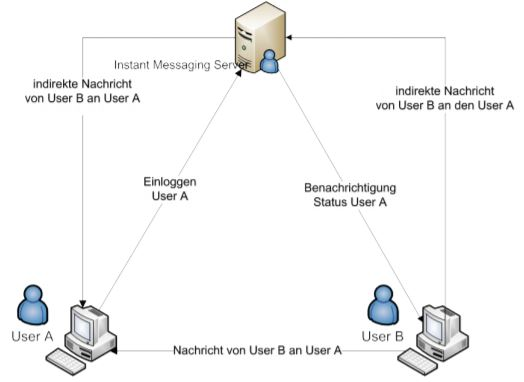
\includegraphics{images/GrundlegendeStrukturIMS}
	\caption{Allgemeine Struktur eines Instant-Messaging-Systems}
	\label{img:StrukturIMS}
\end{figure}

Hat sich der Benutzer mit seinen Login-Daten erfolgreich gegenüber dem Authentifikationsserver authentifiziert, kann er andere, bereits registrierte, Benutzer kontaktieren. Die Verbindungsinformationen wie zum Beispiel IP-Adresse, die dem Client lokal zugewiesene Portnummer und die Kontaktliste (Freunde des Benutzers) werden an den Präsenzserver übermittelt. Dieser ist abhängig von der Implementierungsform ein Teil des \textbf{IM-Servers} oder ein eigenständiger Server. Der Präsenzserver überprüft, welche Benutzer aus der Kontaktliste verfügbar und angemeldet sind. Der Server sendet dem Benutzer die Ergebnisse der Statusüberprüfung zurück. Ist einer der gewünschten Benutzer \glqq online\grqq (verfügbar) kann durch die Auswahl der entsprechenden Kennung eine Verbindung aufgebaut werden und der Nachrichtenaustausch kann beginnen. Das ist möglich, weil der Server dem Sender die IP-Adresse und die Ziel-Portnummer des Kommunikationspartners übermittelt. Die Nachrichten werden direkt zwischen den Clients übertragen oder über den Server zwischen den Kommunikationspartnern übermittelt. Die Art der Übertragung ist von System zu System je nach Realisierung unterschiedlich. Der Kommunikationspfad ist abhängig von der Architektur und dem verwendeten Protokoll. Eine Nachricht kann zentral über den Server vermittelt werden (vgl. \autoref{img:StrukturIMS}-indirekte Nachricht) oder nach dem Peer-to-Peer-Prinzip (vgl. \autoref{img:StrukturIMS}-direkte Nachricht) erfolgen. 

\section{XMPP-Extensible Messaging and Presence Protocol}
\label{sec:XMPP}
\ac{XMPP} bedeutet \textbf{Extensible Messaging and Presence Protocol}. Wird dieses ins Deutsche übersetzt, so entsteht die Bedeutung eines erweiterbares Nachrichten- und Anwesenheitsprotokoll. Eine Definition die \ac{XMPP} sehr gut beschreibt. \ac{XMPP} basiert auf \ac{XML}, welches eine Markup Sprache darstellt. Das Ziel von \ac{XMPP} war ein Protokoll für das Instant Messaging zu entwickeln. Laut dem RFC6120 lässt sich mittels \ac{XMPP} Daten zwischen zwei oder mehreren Netzwerkeinheiten nahezu in Echtzeit austauschen, welches als Vorteil für Sofortnachrichten bezeichnet werden kann. Diesbezüglich nutzt es das Internet und erlaubt den Usern Sofortnachrichten an andere Anwender innerhalb des Internets zu schicken. \ac{XMPP} lässt sich in viele verschiedene Funktionen aufteilen, weshalb der grundlegende Zweck ein anderes Ziel verfolgt. Im einfachsten Sinne ist die Idee von \ac{XMPP} den Austausch von kleinen Teilen strukturierter Daten (\glqq \ac{XML} stanzas\grqq) zwischen einem oder mehreren Netzwerkteilnehmern zu ermöglichen. Primär wird \ac{XMPP} mithilfe einer Client-Server-Architektur implementiert, bei der sich ein Client mit einem Server verbindet, um mit anderen Teilnehmern Daten auszutauschen. Anderseits kann es als Protokoll auch zwischen Servern fungieren. Daraus resultiert der Vorteil nahezu unabhängig von Betriebssystemen und Browsern zu sein. Wird die Client-Server-Architektur implementiert, so ist in der Regel der Ablauf definiert durch folgende Schritte: \cite{RFC6120} 
\begin{enumerate}
	\item Bestimmen der IP-Adresse und des Ports zu dem sich verbunden werden soll 
	\item Eine \ac{TCP} Verbindung öffnen/aufbauen
	\item Öffnen eines \ac{XML}-Streams über \ac{TCP}
	\item Optional: Verwendung von \ac{TLS} für die Verschlüsselung
	\item Verwendung des SASLs Frameworks für die Authentifizierung
	\item Eine Ressource an den \ac{XML} stream anbinden
	\item Austausch unbegrenzter \glqq \ac{XML} stanzas\grqq ()=> kleine Teile strukturierter Daten) mit anderen Netzwerkteilnehmern
	\item Schließen des \ac{XML} streams
	\item Schließen der \ac{TCP} Verbindung
\end{enumerate}
Die folgende \autoref{img:XMPPcommunication} zeigt den Start einer Kommunikation, wie im genannten Ablauf dargestellt, über \ac{XMPP} und den \ac{XML}-streams.

\begin{figure}[h]
	\centering
	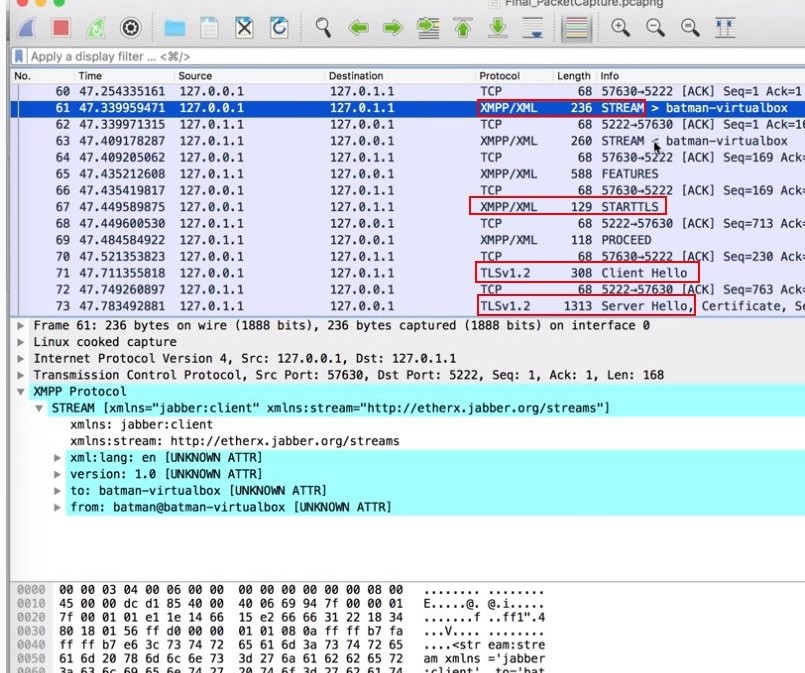
\includegraphics[width=\textwidth]{images/XML_Wireshark}
	\caption{Kommunikationsaufbau des \ac{XMPP}-Protokolls}
	\label{img:XMPPcommunication}
\end{figure} 
\newpage
Für den Austausch von Daten gibt es zwei elementare Konzepte. Zum einen die \ac{XML}-Streams und die \ac{XML}-Stanzas. Diese zwei Konzepte werden definiert um das Verständnis des Datenaustauschs, wie es im obigen Ablauf definiert ist, zu erlangen. Bei dem Austausch der Daten mittels \ac{XML} streams wird von einem Container zwischen den Teilnehmern gesprochen. Der \ac{XML} stream ist durch den \glqq stream header\grqq (z.B. \ac{XML} <stream>) und dem Ende des streams, dargestellt durch \ac{XML} </streams>, eindeutig definiert. Die Anzahl der austauschbaren \ac{XML} Elemente ist unbegrenzt und durch die Lebensdauer des streams definiert. Das \ac{XML} stanza wird nun als diskrete semantische Einheit strukturierter Daten, das von einem Teilnehmer zu einem anderen über den \ac{XML} stream gesendet wird bezeichnet. Das \ac{XML} stanza ist ein direktes Kind-Element des streams. Ein stanza kann wiederum selbst Kind-Elemente enthalten, das den \ac{XML} stream definiert. Im Kern fungiert der \ac{XML} stream wie eine Hülle um alle \ac{XML} stanzas, die während einer Session versendet werden. Ein Aufbau kann wie in der folgenden \autoref{img:StrukturXMLstream} repräsentiert werden. \cite{RFC6120Sec4}
\begin{figure}[h]
	\centering
	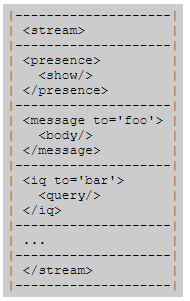
\includegraphics[scale=1.2]{images/XML_Stream}
	\caption{Allgemeine Struktur eines XML streams}
	\label{img:StrukturXMLstream}
\end{figure}
\newpage


\section{Python}
\label{sec:Python}
\newpage

\section{Ejabberd}
\label{sec:ejabberd}
Ejabberd ist einer der bekanntesten freien \ac{XMPP}-Server auf der Welt und kann in vielerlei Hinsicht verwendet werden. Sowohl Großprojekte als auch kleine Instanzen machen sich die Eigenschaften von ejabberd zum Vorteil. Der Start von ejabberd ist dem Jahr 2002 zuzuordnen. Ejabberd ist eine Abkürzung und steht für \glqq Erlang Jabber Daemon\grqq. Wie die Definition zeigt bezieht sich ejabberd auf die Programmiersprache Erlang. Grund hierfür ist, dass die ejabberd Software in Erlang geschrieben ist. Seit dem Start wurde es von Grund auf für die Unternehmensbereitstellung entwickelt, vor allem mit dem Ziel robust zu sein. Aufgrund davon, dass der Fokus auf die Unternehmen lag, war es wichtig die Fehleranfälligkeit von ejabberd zu minimieren. Ein Vorteil der sich bis zum heutigen Zeitpunkt bewahrt hat. Außerdem kann ejabberd die Ressourcen mehrerer geclusterter Systeme nutzen. Des Weiteren besitzt ejabberd die Eigenschaft der Skalierbarkeit, indem die Kapazitäten mit wenig Aufwand erhöht werden kann. Während der Entstehungsphase war das \ac{XMPP}-Protokoll, welches in \autoref{sec:XMPP} beschrieben wird, noch unter dem Namen Jabber bekannt. Ejabberd kann verschieden benutzt werden. Im Fall der Studienarbeit wird die Community Edition von ejabberd benutzt, welche als open source zur Verfügung steht. Neben der Community Edition gibt es auch noch Möglichkeiten einer Business Edition, welches vor allem für die großen Unternehmen mit besserem Support rund um die Uhr und größeren Funktionen konzeptioniert ist. Die Architektur eines ejabberd services erweitert die Kernfunktionen von \ac{XMPP}, welches das Senden von Nachrichten ist, um Faktoren wie die Skalierbarkeit, Konfigurierbarkeit und Fehlertoleranz. Außerdem gilt die Architektur von ejabberd als Modular. Das bedeutet, dass es an den Zweck eines Projektes angepasst werden kann. Die Modularität bringt bspw. Funktionen wie Gruppenchat mit ein. Aufgrund der großen Anzahl an Modulen werden lediglich die Module, die für das Projekt relevant sind aufgelistet.
Relevante Funktionen:
\begin{itemize}
	\item Einzelchat
	\item Gruppenchat (auch als Multi-User-Chat (\ac{MUC}) bezeichnet)
	\item Offline Nachrichten 
	\item Web-Unterstützung
	\item Nachrichtenübermittlungsbestätigung
	\item Übermittlung des Online-Status
	\item Verschlüsselte Übertragung von Nachrichten
	\item Kontaktliste jedes Benutzers
\end{itemize}
Eine wichtige Eigenschaft ist das Authentifizieren von Nutzern, welches ebenfalls von ejabberd unterstützt wird. Dafür kann ejabberd sowohl mit einer internen, als auch mit einer externen Datenbank zusammenarbeiten. Aufgrund der genannten Eigenschaften und Funktionen von ejabberd, werden eine Vielzahl an mögliche Anwendungsgebieten abgedeckt. Während für viele kleine Projekte die interne Datenbank Mnesia ausreichend ist, wird im Rahmen der Studienarbeit mit einer externen Datenbank gearbeitet.\cite{ejabberdDoc}

\section{Chatserver}
\label{sec:Chatserver}

\begin{lstlisting}[language=Python,caption=Example Listing Python,label={lst:Example}]
"""The first step is to create an SMTP object, each object is used for connection 
with one server."""

import smtplib
server = smtplib.SMTP('smtp.gmail.com', 587)

#Next, log in to the server
server.login("youremailusername", "password")

#Send the mail
msg = "
Hello!" # The /n separates the message from the headers
server.sendmail("you@gmail.com", "target@example.com", msg)
\end{lstlisting}


\section{Datenbank}
\label{sec:Datenbank}
Für den Aufbau eines Chatsystems ist ein Datenbanksystem notwendig. Die Datenbank wird benötigt, weil Informationen und Parameter für die Authentifizierung des Benutzers gespeichert werden müssen. Außerdem ist die interne Datenbank Mnesia eines Ejabberd-Chatservers nicht für den Mehrbenutzer-Betrieb ausgelegt. Mnesia ist in der Sprache Erlang entwickelt. Sie besitzt eine weiche Echtzeitfähigkeit und ist auf Geschwindigkeit optimiert \cite{MnesiaDoc}, die verfügbare Speicherkapazität für den Chatserver-Betrieb ist nicht ausreichend für ein Mehrbenutzer-System \cite{ejabberdDoc}. Ein Mehrbenutzer-Betrieb eines Ejabberd-Chatservers benötigt eine Datenbank, in der Nachrichtenverläufe, Kontakte jedes Benutzers und weitere Parameter gespeichert werden können.

\pagebreak

Eine Datenbank beinhaltet eine Sammlung von mehreren Daten, die sich aufeinander beziehen können, und von einem \ac{DBMS} verwaltet werden. Kernkomponente für den Zugriff ist die einheitliche logische Schnittstelle zum \ac{DBMS}. Der Zugriff kann mit dem weitverbreiteten Standard \ac{SQL}, welches im allgemeinen Sinn eine Programmiersprache darstellt, erfolgen. Dafür wird der Datenbank über \ac{SQL} nur mitgeteilt welche Daten benötigt werden. Ein Datenbanksystem muss bestimmte Eigenschaften besitzen, um den Zweck Daten zu speichern und sie wieder abzufragen, zu erfüllen.

\smallskip

\textbf{Eigenschaften:}
\begin{itemize}
	\item Unabhängigkeit von dem physischen Aufbau
	\item Schutz bei (Mehrfach-) zugriff auf Daten
	\item Integrität
	\item Zuverlässigkeit
	\item Ausfallsicherheit
\end{itemize}

Es gibt verschiedene Datenbankmodelle, nach denen eine Datenbankstruktur definiert wird. Die Datenbankmodelle unterteilen sich in relationale, objektorientierte, hierarchische und netzwerkartige sowie in moderne Datenbanken. Für die Projektarbeit wird ein relationales Datenbankmodell verwendet und deshalb dieses Modell genauer vertieft. Dementsprechend sind wichtige Schlüsselbegriffe zu definieren. Eine Tabelle wird ebenfalls als Relation bezeichnet. Eine Zeile der Relation heißt Tupel, die Spalten Attribute. Die Kardinalität entspricht der Anzahl von Tupeln und der Grad bezieht sich auf die Anzahl der Attribute. Ein wesentliche Bestandteil einer relationalen Datenbank ist der Primärschlüssel, welcher zwingend erforderlich ist und eindeutig sein muss. Der Schlüsselbegriff Gebiet bezieht sich auf ein Definitionsbereich eines Attributes, welches alle gültigen Werte für dieses Attribut umfasst. \cite{Schicker2017}

\newpage

\smallskip

\textbf{Beispiel einer Relation:}

\smallskip

\begin{figure}[h]
	\centering
	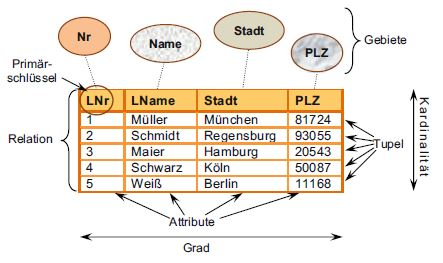
\includegraphics[scale=1.2]{images/RelationMitSchluesselbegriffe}
	\caption{Relation mit Schlüsselbegriffe \cite{Schicker2017}}
	\label{img:RelationDB_Begriffe}
\end{figure}

Eine relationale Datenbank ist definiert als eine Datenbank mit einer Ansammlung von zeitlich variierenden, normalisierten Relationen mit passenden Graden.
\textbf{MySQL} ist eines der weltweit verbreitetsten relationalen Datenbanksysteme, weil sie als Open-Source-Software und als kommerzielle Enterprise-Version verfügbar ist. MySQL wird von allen gängigen Betriebssystemen wie Linux oder Windows unterstützt. Entwickelt wird MySQL von der Oracle Cooperation. Die MySQL-Datenbanken sind relational und orientieren sich an den oben genannten Schlüsselbegriffen, die eine relationale Datenbank definieren. Die MySQL-Datenbank ist in der Software eine Client-Server-Architektur, die aus einem Multi-Threading-Server besteht. Dadurch werden verschiedene Backends, Clientprogramme und Verwaltungswerkzeuge parallel unterstützt.\cite{MysqlDoc}
\newpage

\section{Grafische Benutzeroberfläche}
\label{sec:Benutzeroberfläche}
Eine Grafische Benutzeroberfläche ist im Detail eine Schnittstelle zum Nutzer eines Computers. Die im Hintergrund agierende Software soll mittels Symbole und anderen Elementen bedienbar gemacht werden. Im Englischen wird die Benutzeroberfläche als \ac{GUI} bezeichnet, welches im weitere Verlauf ebenfalls als Bezeichnung verwendet wird. Allgemein besitzt eine \ac{GUI} Bedien- und Steuerelement die mit der im Hintergrund laufenden Software interagiert. Der Einsatz einer \ac{GUI} liegt an der Usability, welches die Benutzerfreundlichkeit beschreibt. Eine \ac{GUI} soll demnach dem User die Möglichkeit geben, die Software auch ohne großen Aufwand bedienen zu können. Eine Eigenschaft die heutzutage nahezu jedes Programm beinhalten muss. %TODO
\url{https://de.wikipedia.org/wiki/Grafische_Benutzeroberfl%C3%A4che}
	
Im Rahmen der GUI-Programmierung müssen mehrere Aspekte berücksichtigt werden um die Usability zu erfüllen. Dafür werden die Aspekte in 8 goldene Regeln zusammengefasst, die bei der Entwicklung einer GUI berücksichtigt werden sollten.
\begin{enumerate}
	\item Strebe nach Konsistenz
	\item Sorge für universelle Bedienbarkeit
	\item Biete informative Rückmeldung
	\item Entwerfe abgeschlossene Dialoge
	\item Biete einfache Fehlerbehandlung
	\item Lass die Einfache Umkehrung von Aktionen zu
	\item Vermittle ein Gefühl der Kontrolle
	\item Entlaste das Kurzzeitgedächtnis
\end{enumerate}
Im Folgenden wird kurz auf die 8 Regeln eingegangen, damit eine Verbindung zur Umsetzung der \ac{GUI} in \autoref{subsec:EntwicklungGUI} entsteht.

Der erste Punkt, \textbf{Strebe nach Konsistenz}, befasst sich bspw. mit dem Erscheinungsbild einer Seite. Die Seite sollte dem Aspekt zur Folge die Elemente, wie einen Button, immer an der gleichen Stelle positionieren.

Der nächste Punkt, \textbf{Sorge für universelle Bedienbarkeit}, beinhaltet Anforderungen an die Vielfalt an Nutzer. Somit sollte jeder Nutzer die Bedienung, Kürzel usw. ohne Einschränkungen verstehen können.

Ein Nutzer verlangt nach ausreichendem Feedback, die vor allem informativ und in vielen Fällen auch hilfreich sind. Ein Fakt der im dritten Punkt, \textbf{Biete informative Rückmeldung}, behandelt wird

Der vierte Punkt, \textbf{Entwerfe abgeschlossene Dialoge}, umfasst die Führung eines Nutzers, bspw. durch eine Verkaufsprozess. Zu jedem Zeitpunkt soll der Nutzer wissen, in welchem Prozess er sich befindet.

Um die Bedürfnisse der Nutzer gerecht zu werden muss wie in Punkt fünf, \textbf{Biete einfache Fehlerbehandlung}, definiert, die Fehler mit nützlichen Informationen für den Nutzer ausgestattet werden. Außerdem muss ein Ausweg in den normalen Programmablauf gewährleistet sein.

Ein Nutzer soll mit Punkt sechs, \textbf{Lass die Einfache Umkehrung von Aktionen zu}, die Möglichkeit haben kleine Ereignisse rückgängig zu machen.

Der siebte Punkt, \textbf{Vermittle ein Gefühl der Kontrolle}, beinhaltet die Aktion und Reaktion. Demnach soll die Software auf eine Aktion des Nutzers reagieren und nicht andersrum. 

Der letzte Punkt, \textbf{Entlaste das Kurzzeitgedächtnis}, soll gewährleisten, dass die GUI schlicht und einfach gehalten werden soll. Ein Nutzer sollte sich keine große Anzahl an Informationen merken müssen um einen Aktion auszuführen.
\cite{UI8Regeln2019}

Aufgrund der 8 goldenen Regeln, kann im Umsetzungsprozess auf diese zurückgegriffen werden um eine benutzerfreundliche Oberfläche zu erstellen. Im folgenden Abschnitt wird auf die \ac{GUI}-Programmierung mit Python eingegangen.


\subsection{GUI-Programmierung mit Python}
\label{subsec:GuiPython}
Mit Python als Programmiersprache kommen mehrere Module, welche für die Grafische Benutzeroberfläche benutzt werden können, einher. Dementsprechend wird in diesem Abschnitt ein Einblick in die Möglichkeiten, passend zur Aufgaben- und Problemstellung, gegeben werden. Abhängig von den Erkenntnissen folgt eine Entscheidungsmatrix um das passende Modul für das Projekt auszuwählen.

Die \ac{GUI}-Programmierung bei Python unterscheidet sich im Konzept nicht allzu sehr von anderen Programmiersprachen. Neben Schaltflächen stehen auch Fenster oder Menüs als Komponenten zur Verfügung. Angeordnet können diese in sogenannten Container. Für eine geeignete Anwenderschnittstelle müssen die Komponenten in die Container integriert werden. Hinzukommt ein äußerer Container, auch als Frame bezeichnet, ein Layout-Manager und eine Implementierung damit Aktionen durch Komponenten ausgelöst werden können. Wie im \autoref{sec:Benutzeroberfläche} erläutert, verfolgt eine \ac{GUI} mehreren Regeln. Demnach gibt es für die Programmierung einer grafischen Benutzeroberfläche vielerlei Möglichkeiten. In Python werden \ac{GUI} Frameworks angeboten, die eine Programmierung erleichtern sollen. Diese Frameworks können sich in der Art und der Verwendung unterscheiden. Aufgrund davon muss erst die Art des Frameworks ermittelt werden. Dafür wird eine Entscheidungsmatrix erstellt, basierend auf Faktoren, die passend zum Projekt Auswirkungen haben.\cite{Steyer2018} \\
Die nachfolgende \autoref{tab:EntscheidungsmatrixFrameworkart} spiegelt die Ergebnisse eines Vergleichs zwischen den Tool-Frameworks und den Web-Frameworks von Python wieder. Die Kriterien orientieren sich am Projekt und werden nachfolgend erläutert. Die \textbf{Nutzerfreundlichkeit} umfasst wie verständlich ein GUI mithilfe des Tools aufgebaut werden kann. Außerdem beinhaltet das Kriterium auch die Möglichkeiten des Tools auf die Nutzerfreundlichkeit einzugehen. Die \textbf{Schwierigkeit} orientiert sich an der Implementierung. Dabei geht darum wie leicht, schnell und komfortabel die Frameart integriert werden kann. Unabhängig von der Schwierigkeit geht es bei der \textbf{Umsetzbarkeit} um die Mittel, welche für eine Umsetzung benötigt werden, sowie auch um den Aufwand bei der Umsetzung. Die \textbf{Kompatibilität} umfasst die Unabhängigkeit von Betriebssystemen, Browsern usw. Standard für eine grafische Oberfläche bildet auch das \textbf{Design}. Demnach geht es um die Möglichkeiten eines guten Erscheinungsbilds der Oberfläche mit dem entsprechenden Framework. Das letzte Kriterium, \textbf{Verwendungszweck}, bildet die Verbindung zum Projekt. Dabei wird analysiert wie die Frameworkart zum Zweck des Projektes passt. Die Gewichtung der Kriterien innerhalb der \autoref{tab:EntscheidungsmatrixFrameworkart} sind der TABELLE des ANHANGS zu entnehmen.
\renewcommand{\arraystretch}{2}
\begin{table}[h]
\centering
	\begin{tabular}{l|c|c|c}
		& & \multicolumn{2}{c}{Arten einer Python-GUI} \\
		Kriterien & Gewichtung & Tool-Framework & Web-Framework \\
		\hline
		Nutzerfreundlichkeit & 33\% & 2 & 2 \\
		\hline
		Schwierigkeit & 7\% & 2 & 1,7  \\
		\hline
		Umsetzbarkeit & 13\% & 2 & 2,2\\
		\hline
		Kompatibilität & 13\% & 2,2 & 1,7 \\
		\hline
		Design & 7\% & 2 &  2\\
		\hline 
		Verwendungszweck & 27\% & 2,5 & 1,5 \\
		\hline
		\textbf{Gesamtwertungszahl} & \textbf{100\%} & \textbf{2,161} & \textbf{1,831} \\
	\end{tabular}
\caption{Entscheidungsmatrix der Frameworkart}
\label{tab:EntscheidungsmatrixFrameworkart}
\end{table} \\
Die \autoref{tab:EntscheidungsmatrixFrameworkart} bildet eine Hilfestellung zur Entscheidung einer passenden Frameworkart für das Projekt. Die Bewertung der Tools entsprechend der Kriterien folgt dem Benotungsschema der akademischen Bildung. Demnach ist eine 1 sehr gut und eine 6 ungenügend. Im Kriterium Nutzerfreundlichkeit schließen beide Frameworks mit der gleichen Note ab, da die Nutzerfreundlichkeit abhängig vom Designstil ist und bei beiden Frameworks umgesetzt werden kann. Die Schwierigkeit, wie das Kriterium in der Einführung definiert wurde, bekommt beim Web-Framework eine bessere Bewertung. Grund hierfür ist, dass für das Web-Framework überwiegend keine aufwändigen Module in Python benötigt werden. Die Gestaltung erfolgt nämlich über HTML und CSS, welche dann mit einem schlichten Modul verknüpft bzw. aufgerufen werden können. Aufgrund von Vorkenntnissen sowohl in HTML als auch in CSS wird die Schwierigkeit für das Web-Framework besser bewertet. Bei der Umsetzbarkeit steht das Tool-Framework aufgrund der Verwendung eines gesamten Moduls besser da. Ein Web-Framework bringt HTML, CSS und das Modul mit was ein größeren Umfang bedeutet. Vor allem muss der Programmierer mit allen Elementen umgehen können, weshalb eine Umsetzung schwieriger sein könnte. In der Kompatibilität wird das Web-Framework aufgrund der Unabhängigkeit bezüglich des Betriebssystem besser bewertet. Außerdem kann eine ausgelieferte HTML-Seite von nahezu allen Browsern gelesen werden, und eine Möglichkeit die Lösung auf mobilen Endgeräten zu benutzen ist ebenfalls enthalten. Im Design unterscheiden sich die Frameworkarten nicht. Beide bieten vielerlei Möglichkeiten im Bezug auf die Gestaltung. Aufgrund des Projektes einen Chat über \ac{XMPP} und ejabberd zu realisieren wird schon hauptsächlich das Internet genutzt. Dadurch bietet es sich den Server eine HTML-Seite ausliefern zulassen. Aus diesem Grund wird das Web-Framework im Rahmen dieses Kriteriums besser bewertet. Anhand der Gesamtwertungszahl entsprechend der Benotung und der Gewichtung sind beide Frameworks zu empfehlen, dennoch schließt das Web-Framework besser ab, weshalb im weiteren Verlauf ein Web-Framework zum Einsatz kommen soll. \cite{FrameworkOverview} \cite{WebFramework}\\
Mit diesem Ergebnis müssen die verschiedenen Möglichkeiten eine Web-Framework in Bezug auf Python analysiert und bewertet werden. Auch in diesem Fall liefert eine Entscheidungsmatrix ein aufschlussreiches Ergebnis. Die Definition der selben Bewertungskriterien sind der Einführung der \autoref{tab:EntscheidungsmatrixFrameworkart} zu entnehmen. Kriterien wie Umfang und Komplexität werden in die Betrachtung miteinbezogen. Der \textbf{Umfang} spiegelt die Möglichkeiten und Größe im Aufbau des Tools wieder. Die \textbf{Komplexität} befasst sich im Grunde mit dem Aufwand einer Implementierung sowie auch die Hilfestellungen durch geeignete Dokumentationen. Das Bewertungsschema orientiert sich ebenfalls an der \autoref{tab:EntscheidungsmatrixFrameworkart}.\\
\begin{table}[h]
	\centering
	\begin{tabular}{l|c|c|c|c|c}
		Kriterien & Gewichtung & Django & Flask & CherryPy & Bottle\\
		\hline
		Umfang & 17\% & 1,5 & 2 & 2 & 2,5 \\
		\hline
		Schwierigkeit & 17\% & 2,5 & 1,7 & 2,2 & 2 \\
		\hline
		Komplexität & 33\% & 2,2 & 1,7 & 2 & 1,7 \\
		\hline
		Verwendungszweck & 33\% & 2 & 2 & 2 & 2,2 \\
		\hline
		\textbf{Gesamtwertungszahl} & \textbf{100\%} & \textbf{2,067} & \textbf{1,850} & \textbf{2,033}  & \textbf{2,050} \\
	\end{tabular}
	\caption{Entscheidungsmatrix eines Web-Frameworks}
	\label{tab:EntscheidungsmatrixWebFramework}
\end{table}Die Gesamtwertungszahl, welches der \autoref{tab:EntscheidungsmatrixWebFramework} entnommen werden kann, liefert ein knappes Ergebnis. Demnach bietet sich Flask am besten als Framwork einer grafischen Oberfläche an. Im Umfang setzt sich das Tool Django gegen die Konkurrenten durch, da es aufgrund seiner Größe vielerlei Möglichkeiten mitbringt. Während die anderen Tools überwiegend als Mikroframework bezeichnet werden zeichnet sich Django als Full-Stack/high-level Framework aus. Ebenfalls ein Grund weshalb die Schwierigkeit bei Django mit einer 2,5 bewertet wurde. Ein Mikroframework bildet in der Hinsicht die leichtere und schnellere Variante. Die Komplexität wurde vor allem bei Flask und Bottle gut bewertet. Grund hierfür ist unter anderem eine geringere Komplexität durch Möglichkeiten einer schlichten Implementierung. Außerdem bietet bspw. Flask eine sehr gute Dokumentation, welche die Komplexität verringern. Der Verwendungszweck ist nahezu gleichbleibend, da alle Frameworks genutzt werden können um das Projekt umzusetzen. Ausschließlich bei Bottle ist überwiegend die Rede von einem Framework das vor allem zur Einführung in das Themengebiet der Programmierung grafischer Oberflächen mit eine Web-Framework benutzt wird. Anhand des Ergebnisses und der sehr guten Dokumentation wird Flask als Web-Framework zum Einsatz kommen.\cite{BottleDoc} \cite{CherryPyDoc} \cite{DjangoDoc} \cite{FlaskDoc}

\subsection{Flask}
\label{subsec:Flask}
Wie unter \autoref{subsec:GuiPython} beschrieben, wird im Rahmen der Studienarbeit Flask verwendet. Es ist ein Python Web-Framework welches eine Schnittstelle zum Webserver bildet. Bekannt ist Flask durch die Eigenschaft schnell und leicht eine minimale Anwendung zu implementieren und diese bei Bedarf in der Größe zu skalieren. Für die Verwendung von Flask sind zwei Bibliotheken wichtig. Bei diesen handelt es sich zum einen über die \ac{WSGI}-Bibliothek Werkzeug und der Template-Bibliothek Jinja2. Module die standardmäßig von Flask verwendet werden. Flask bildet im Grunde das Bindeglied zwischen den Modulen und erlaubt es bspw. mithilfe des \textbf{Routings} an bestimmten Endpunkten eine \ac{HTML}-Datei zu rendern. Ein Möglichkeit dafür zeigt das folgende \autoref{lst:FlaskMinApp}.
\begin{lstlisting}[language=Python,caption=Example Listing of Flask Python,label={lst:FlaskMinApp}]
from flask import Flask
app = Flask(__name__)

@app.route('/')
def homepage():
	 return render_template('homepage.html')
\end{lstlisting}
Das \autoref{lst:FlaskMinApp} spiegelt das Routen sowie das Rendern einer \ac{HTML}-Datei von Python wieder. Aufgrund des Paketverwaltungsprogramm pip kann Flask komfortable installiert werden. Dementsprechend wird Flask in der ersten Zeile importiert, dann einer Anwendung zugeordnet und eine Route definiert. Nun besitzt Flask vielerlei Möglichkeiten, so kann bspw. je nach Anfrage (POST, GET, usw.) differenziert werden. In dem Zusammenhang kommt eine weiterer möglicher Vorteil von Flask zum Einsatz. Dieser beinhaltet die Möglichkeit einen Webserver, den Flask zur Verfügung stellt, im Entwicklungsmodus zu starten und aktuelle Code-Zeilen zu testen.
Flask ist also nicht zuständig für die Gestaltung der grafischen Oberfläche sondern benutzt sogenannte \textbf{Templates} in Form von HTML-Datei, die eine Webseite aufbauen. Für eine dynamische Webanwendung und den gestalterischen Aspekten sind statische Dateien, wie z.B. \ac{CSS}, notwendig. Aus diesem Grund benötigt Flask eine vorgegebene Ordnerstruktur, welche der nachfolgenden \autoref{img:TreeFlaskOrdnerstrukt} entnommen werden kann.
\begin{figure}[h]
	\centering
	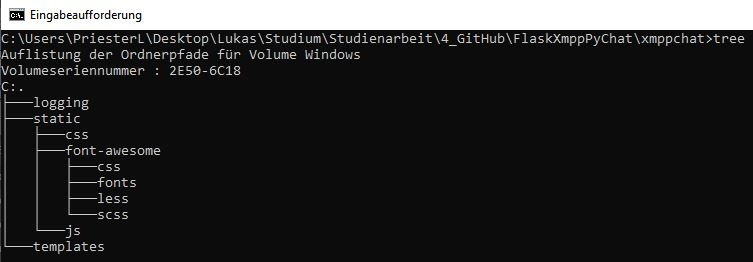
\includegraphics[width=\textwidth]{images/TreeFlaskOrdnerstrukt}
	\caption{Ordnerstruktur unter Flask}
	\label{img:TreeFlaskOrdnerstrukt}
\end{figure}
Für die grafische Benutzeroberfläche würden diese Elemente ausreichen um eine simple Webseite aufzubauen, mit den \ac{HTML}- und \ac{CSS}-Dateien zu verknüpfen, über das Routen die Seite zu rendern und letztendlich, über den von Flask gestellten Webserver, zu testen. Dennoch bietet Flask mehr Möglichkeiten auch im Zusammenhang des Projektes. Zum Beispiel kann in Flask mit redirects, sessions, cookies, Datenbanken und vieles mehr gearbeitet werden. Dabei verfolgt Flask das Ziel dem Anwender nichts vorzuschreiben, dadurch ist er unabhängiger und kann auf vielerlei Erweiterungen zugreifen. Bei der Anbindung einer \textbf{Datenbank} gibt es so die Möglichkeit bspw. eine MySQL, PostgreSQL, SQLite oder andere Datenbanken zu verwenden. In diesem Zusammenhang bietet Flask das Modul Flask-SQLAlchemy, welches der Flask-Anwendung das SQLAlchemy Paket hinzufügt. Ziel ist es die Verwendung von SQLAlchemy mit Flask zu vereinfachen. Das Paket gilt als \ac{ORM}, und bietet die Möglichkeit high-level Operationen in Datenbank-Kommandos zu übersetzen. Im Rahmen der Studienarbeit wird ebenfalls die Erweiterung Flask-SQLAlchemy angewendet. Demnach kann eine Implementierung, einer minimalen Anwendung mit Datenbank, wie im folgenden \autoref{lst:SQLAlchemyMinApp} dargestellt, aussehen.
\begin{lstlisting}[language=Python,caption=Example Listing of Flask-SQLAlchemy,label={lst:SQLAlchemyMinApp}]
from flask import Flask
from flask_sqlalchemy import SQLAlchemy

app = Flask(__name__)
app.config['SECRET_KEY'] = os.urandom(24) #secret key of app
app.config['SQLALCHEMY_DATABASE_URI'] = config.get('SQLALCHEMY_DATABASE_URI')

db = SQLAlchemy(app)

class User(db.Model):
	user_id = db.Column(db.Integer, primary_key=True, autoincrement=True)
	username = db.Column(db.String(25), unique=True, nullable=False)
	email = db.Column(db.String(35), unique=True, nullable=False)
	passwd = db.Column(db.String(112), nullable=False)
	
	def __init__(self, user, email, passwd):
		self.username = user
		self.email = email
		self.passwd = self.set_password(passwd)
	
	def get_id(self):
		return (self.user_id)

@app.route('/login')
def login():
	user = User(req_content["username"], req_content["eMail"], req_content["password"])
	db.session.add(user)
	db.session.commit()
	return render_template('homepage.html')
\end{lstlisting}
Neben dieser Erweiterung bietet Flask auch ein Modul im Rahmen eines Login, welcher ebenso für das Projekt relevant ist, an. Dafür kann der Login Manager aus Flask-Login verwendet werden. Dieser beinhaltet nützliche Funktionen auf die innerhalb der Anwendung zugegriffen werden kann. Für den Login-Manager werden sessions benötigt, welche ebenfalls importiert werden müssen. Das liegt an der Authentifizierung, weshalb ein sicherer Schlüssel, wie er im \autoref{lst:LoginManagerMinApp} dargestellt ist, erzeugt werden muss.
\begin{lstlisting}[language=Python,caption=Example Listing of Flask-Login,label={lst:LoginManagerMinApp}]
from flask import Flask
from flask_login import LoginManager, login_required, login_user, logout_user, current_user

app = Flask(__name__)

login_mgmt = LoginManager(app)
login_mgmt.login_view = 'login' # name of callback method if unauthorized user accessed a login protected site

@app.route("/login", methods=['GET', 'POST'])
def login():
	if current_user.is_authenticated:
		return redirect(url_for('gochat'))
	login_user(user)
	return render_template('login.html')
\end{lstlisting}
Diese beispielhafte Listings wichtiger Module zeigen die Möglichkeiten des Web-Frameworks. Mitunter der Grund für die Verwendung von Flask. Außerdem sind nur wenige Module dargestellt. Weitere Erweiterungen, die im Rahmen des Projektes eingesetzt werden folgen bei der Umsetzung. Diese dargestellt bilden lediglich die theoretische Grundlagen um das Funktionsprinzip von Flask zu erläutern.
\pagebreak

\section{HTML, CSS und JavaScript als Werkzeuge der Webentwicklung}
Wie unter \autoref{subsec:Flask} erläutert, benötigt Flask für die grafische Oberfläche weitere Elemente, die das Erscheinungsbild aufbauen, gestalten und mit Dynamik verknüpfen. Dafür werden die Werkezeuge des Webdesign benötigt. Diese umfassen \ac{HTML}, \ac{CSS} und JavaScript.

\textbf{\ac{HTML}}\\
Das Internet mit seinen Funktionen Text-, Bild, Sound und weiteres abzubilden oder zu übertragen basiert auf einem gemeinsamen Standard. Dieser ist unter dem Namen Hypertext Markup Language \ac{HTML} bekannt, welcher zu deutsch unter einer Auszeichnungssprache zu verstehen ist. Konkret bezieht sich HTML auf Hypertexte die per Definition die Verlinkung zwischen Texte mithilfe von Hyperlinks bezeichnen. \ac{HTML} als Markup Language entstand schon 1989 und diente zur Beschreibung und Verlinkung von Text. Mit \ac{HTML}5, welches ergänzend zur ersten Variante auch Audio- oder Videodateien an die Webseite binden kann, befindet sich die aktuellste Version im Umlauf. Während eine Weboberfläche unabhängig vom Betriebssystem ist, spielt die Verwendung von Browsern, die ihre eigenen HTML-Parser besitzen, eine bedeutsame Rolle. Aus diesem Grund können vom Webserver ausgelieferte \ac{HTML}-Dateien bei einer geringen Anzahl an Browsern Probleme bereiten. Innerhalb eines \ac{HTML}-Dokuments ist vor allem das Grundgerüst und der Aufbau relevant. Demnach werden die Elemente einer Webseite mit Sprachelementen, sogenannten Tags, beschrieben. Der Aufbau eines Grundgerüst ist in der \autoref{img:GrundgeruestHTML} dargestellt.
\begin{figure}[h]
	\centering
	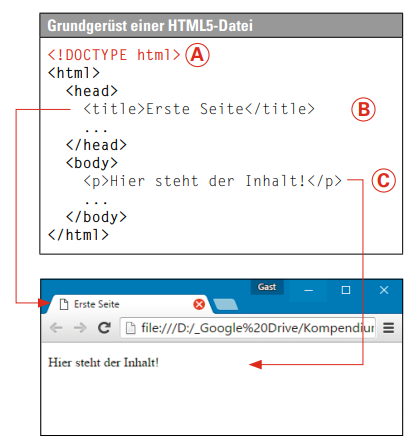
\includegraphics[scale=1.3]{images/HTML_Grundgeruest}
	\caption{Grundgerüst einer HTML-Datei} %TODO Quellenangabe
	\label{img:GrundgeruestHTML}
\end{figure}
\\Der \autoref{img:GrundgeruestHTML} sind die 3 wichtigen Tags (html, head, body) eines Standard \ac{HTML}-Dokumentes sowie der unter A angegebenen Dokumenttyp zu entnehmen. Während in vielen Programmiersprachen die Syntax umfassend groß sein kann, ist die Grammatik bei HTML sehr schlicht. Für die Korrektheit sind daher die genannten Tags bedeutend. Außerdem werden überwiegend Verschachtelung bei der Darstellung einer Webseite benötigt. Für weiteren Einfluss auf die Tags können sogenannte Attribute, wie in der folgenden \autoref{img:HTMLattribute} dargestellt, den Tags zugeteilt werden. 
\begin{figure}[h]
	\centering
	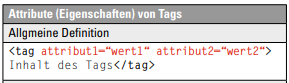
\includegraphics[scale=2.5]{images/HTMLattribute}
	\caption{Attribut eine \ac{HTML}-Tags} %TODO Quellenangabe
	\label{img:HTMLattribute}
\end{figure}
\\Eine \ac{HTML}-Datei entsteht also vor allem durch Tags. Während nun das Dateiformat als reine Textdatei vorliegt, entstehen Fragen über die gestalterischen Aspekte wie z.B. Farben, Grafiken, Videos oder ähnliches. Hauptsächlich werden diese Aspekte innerhalb einer \ac{CSS}-Datei behandelt, dennoch gibt es dafür auch Punkte, die in einer \ac{HTML}-Datei zu beachten sind. Um beispielsweise Grafiken oder Videos, die sich innerhalb eines anderen Unterordners befinden, zu integrieren, muss auf diese referenziert werden. Hierfür bietet \ac{HTML} die absolute und relative Referenz. Eine absolute Referenz, wie z.B. \textit{C:/Dokumente/Mustermann/ Eigene Dateien/Webseiten/button.gif}, wird aufgrund der Abhängigkeit zum User des Computers nicht verwendet. Für die relative Referenz ist wiederum eine einheitliche Ordnerstruktur wichtig, da der Pfad von dem Speicherort der \ac{HTML}-Datei angegeben wird. Diese Struktur kann, wie in der folgenden Abbildung dargestellt, aussehen.
\begin{figure}[h]
	\centering
	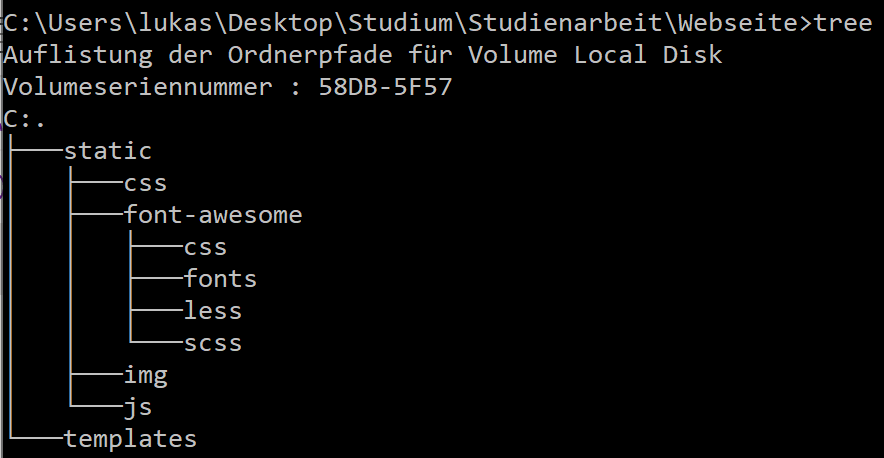
\includegraphics[scale=0.8]{images/TreeHTMLStruktur}
	\caption{Ordnerstruktur bei der Webentwicklung} %TODO Quellenangabe
	\label{img:TreeHTMLStruktur}
\end{figure}
\\Demnach würde die \ac{HTML}-Datei in dem Ordner \textit{templates} liegen und die Bilder im Ordner \textit{static/img}, welcher über die relative Referenz unabhängig vom Betriebssystem und ähnliches erreicht werden kann. Je nach Dateityp orientieren sich auch die Tags innerhalb des \ac{HTML}-Dokumentes danach. Für eine Grafik gibt es daher den <img>-Tag, der die Referenz zum Bild enthält. Mit der Webentwicklung wird das Ziel verfolgt Inhalt und Gestaltung strikt voneinander zu trennen. Daher werden \ac{CSS}-Dateien, die sich mit dem Design befassen, benötigt.

\textbf{CSS:}\\
Die Dateien, die als \ac{CSS} deklariert werden, übernehmen die gestalterischen Aspekte, die ein \ac{HTML}-Dokument nicht erfüllen kann. Neben Designvarianten bietet \ac{CSS} auch die Möglichkeit die Webseite an das jeweilige Endgerät, unterschiedlicher Auflösung, anzupassen. Wie schon für die \ac{HTML}-Dateien gilt auch für \ac{CSS}, dass Attribute nur von bestimmten Browsern akzeptiert werden. Daher gehört zur Webentwicklung ein ausgiebiges Testen dazu. Eine \ac{CSS}-Datei sollte Regeln folgen um Probleme, die im Zusammenhang mit dem HTML-Dokument auftreten können, zu verhindern. Die Grundregel bezieht sich auf den Ort der \ac{CSS}-Definition. Diese kann zum Einen in einer externen Datei, intern in einem eigenen Tag, oder integriert in den \ac{HTML}-Tag erfolgen. Dies ist unter anderem relevant wenn mehrere \ac{CSS}-Dateien zum Einsatz kommen, da die verschieden Orte durch verschiedene Prioritäten geprägt sind. Generell wird die \ac{CSS}-Definitionen in eine eigene Datei ausgelagert um das Design und die \ac{HTML}-Datei zu trennen. Die \autoref{img:CSSrules} stellt dar wie eine \ac{CSS}-Definition aufgebaut ist.
\begin{figure}[h]
	\centering
	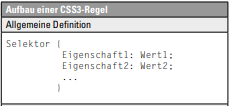
\includegraphics[scale=2.5]{images/CSS_Definition}
	\caption{Aufbau einer \ac{CSS}-Regel} %TODO Quellenangabe
	\label{img:CSSrules}
\end{figure}	
\\Der Aufbau besteht grundlegend aus einem Selektor, dem seine Eigenschaften bearbeitet werden sollen. Damit die Auswirkungen erkennbar werden muss die \ac{CSS}-Datei mit dem HTML-Dokument verknüpft werden. Dies erfolgt innerhalb des Head-Tags in der \ac{HTML}-Datei mithilfe des link-Tags \textit{<link rel=\dq sytlesheet\dq \;type=\dq text/css\dq \;href=\dq design.css\dq>}. Der Selektor befindet sich immer vor einer geschweiften Klammer und kann unterschiedlich verwendet werden. Aufgrund der Verbindung zur HTML-Datei hängt der Selektor vom \ac{HTML}-Tag ab. Wird bspw. ein Button in dem \ac{HTML}-Tag als Klasse definiert so erfolgt der Zugriff über den Punkt. Wird jedoch der Button mit einer ID ausgestattet, so muss mit dem Hashtag darauf zugegriffen werden. Die nachfolgende Abbildung zeigt diese Varianten.
\begin{figure}[h]
	\begin{minipage}[c]{.4\textwidth}
		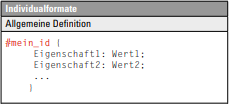
\includegraphics[width=\textwidth]{images/CSSID}
		\caption{Zugriff über ID} %TODO Quellenangabe
		\label{img:CSSID}
	\end{minipage}
	\hspace{.1\linewidth}% Abstand zwischen Bilder
	\begin{minipage}[c]{.4\textwidth}
		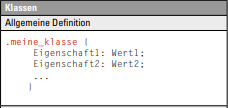
\includegraphics[width=\textwidth]{images/CSSKlasse}
		\caption{Zugriff über Klasse} %TODO Quellenangabe
		\label{img:CSSClass}
	\end{minipage}
\end{figure}
Für die Eigenschaften bietet sich mit der dritten Version von \ac{CSS} (\ac{CSS}3) eine Vielzahl an Möglichkeiten. Grundlegend kann jedes Element mithilfe der \ac{CSS}-Datei bearbeitet werden. Die Eigenschaften sind bspw. Gegliedert unter Typografie, Farbe, Abstände, Tabellen und vieles mehr. In diesem Zusammenhang ist auch die Verwendungen von Maßeinheiten bedeutsam. Mit \ac{CSS}3 werden viele verschiedene Ma"seinheiten unterstützt worüber die Abbildung einen genaueren Überblick gibt.
\begin{figure}[h]
	\centering
	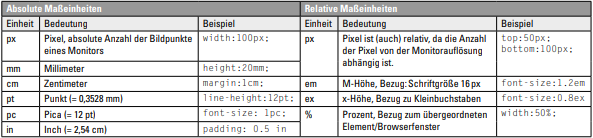
\includegraphics[scale=1.8]{images/CSSmasseinheiten}
	\caption{Ma"seinheiten innerhalb der Webentwicklung} %TODO Quellenangabe
	\label{img:CSSmasseinheiten}
\end{figure}
\ac{CSS} verwendet die Selektoren und wendet auf diesen die definierten Eigenschaften an. Nebenbei bietet \ac{CSS} die Möglichkeit an ein Layout zu erstellen. Dafür ist das sogenannte Boxmodell ausschlaggebend. Dieser ist definiert, die Elemente als eine Box mit Eigenschaften zu betrachten. Demnach gibt es in dem Zusammenhang vielerlei Möglichkeiten eine Box an die richtige Position, sowie mit der richtigen Größe abzubilden. Die Boxen können mit absoluten Werten definiert werden. Mit relativen Werten, welche Prozentwerte enthalten, können die Boxen sich in Abhängigkeit des Browserfensters ändern. Mit \ac{CSS}3 gibt es auch die Möglichkeiten flexible Boxen zu verwenden. Dadurch werden die Boxen unabhängig von der Position und Anordnung spalten- oder zeilenweise an den zur Verfügung gestellten Platz angeordnet. Bei der Betrachtung des Layouts spielt ebenfalls das Endgerät eine Rolle. In dem Zusammenhang können \textbf{Media Queries} zum Einsatz kommen. Diese bieten die Option, Eigenschaften eines Selektors entsprechend der angegebenen Pixel zu ändern.
\begin{figure}[h]
	\centering
	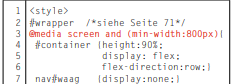
\includegraphics[scale=2.8]{images/MediaQbsp}
	\caption{Beispiel eines Media Queries} %TODO Quellenangabe
	\label{img:/MediaQbsp}
\end{figure}
\\Die Abbildung stellt dar wie die Media Queries eingesetzt werden können. Die Definition erfolgt entweder in der \ac{CSS}-Datei oder in dem Style-Tag einer \ac{HTML}-Datei. Mit diesen Grundlagen lassen sich Seiten gestalterisch anpassen und auf mehreren mobilen Endgeräten ausgeben. Wird Content benutzt der sich ggf. zur Laufzeit ändert, wird überwiegend auf das dritte Element der Webentwicklung zurückgegriffen. Dabei geht es um JavaScript.\cite{buhler2017html5}

\textbf{JavaScript}\\
JavaScript verfolgt das Ziel interaktive oder dynamische Elemente auf der Webseite zu integrieren. Es ist eine Skriptsprache, die überwiegend auf Seiten des Clients eingesetzt wird. Der Code kann direkt über den Browser ausgeführt werden, da ein heutiger Browser einen Interpreter für die Skriptsprache besitzt. Dadurch ist JavaScript von den heutigen Browsern abhängig, weshalb ausgiebige Tests auf verschiedene Browsern erfolgen muss. Mit JavaScript ergeben sich Möglichkeiten Probleme bzw. Schwierigkeiten dynamisch zu lösen. Ein beliebter Fall als Beispiel ist die Formularüberprüfung. Hierbei kann JavaScript die Korrektheit noch auf Seiten des Clients überprüfen und erst nach Abschluss dem Server übertragen. Dadurch können unnötige Datenübertragungen verhindert werden. Eine Schwierigkeit die JavaScript birgt ist die Ausschaltfunktion in den meisten Browsern. Besitzt eine Webseite eine große Anzahl an JavaScript Code so kann durch Deaktivierung im Browser mancher Content nicht mehr funktionieren. Wie mit der Integration von CSS gibt es auch bei JavaScript die Möglichkeit es innerhalb der HTML-Datei oder in einer externen Datei zu verwenden. Im Falle der internen Lösung gibt es den <script>-Tag, der eine JavaScript-Code enthalten kann. Das nachfolgende \autoref{lst:JavaScriptExample} stellt dar, wie so ein JavaScript in den HTML-Body integriert werden kann.
\begin{lstlisting}[language=HTML,caption=Example Listing of JavaScript-Code,label={lst:JavaScriptExample}]
<div class="Login_succeeded">
<script>
document.write("Your Login was succesful");
</script>
</div>
\end{lstlisting}
Das Beispiel bildet ein simpler Fall von JavaScript ab. Der Code erzeugt lediglich ein Text in der HTML-Klasse. Eine der beliebtesten Verwendungen von JavaScript sind Fenster, die zur Benachrichtigung oder Warnung benutzt werden. In Verbindung mit Event-Handler, die auf bestimmte Ereignisse reagieren, kann so, je nach Anwendung Fenster oder andere Elemente erzeugt werden. Ein Beispiel für solch ein Event-Handler wäre das "onclick". Dadurch lässt sich JavaScript-Code erst ausführen wenn bspw. auf ein Button geklickt wird. Neben Fenstern gibt es zahlreiche weitere Verwendungsmöglichkeiten, wie zum Beispiel Formulare, Textfelder, Checkboxen usw. Eine besondere Variante von JavaScript ist \textbf{\ac{Ajax}}, welches ein weiteres wichtiges Feature mit in die Webentwicklung einbringt. \ac{Ajax} kommt vor allem zum Einsatz, wenn es um Elemente geht die nicht durch eine Aktualisierung des Browser ausgelöst werden sollen. \ac{Ajax} ermöglicht in solch einem Fall die dynamische Anfrage. Die Nachfolgende Abbildung erklärt das Funktionsprinzip von \ac{Ajax} sehr genau.
\begin{figure}[h]
	\centering
	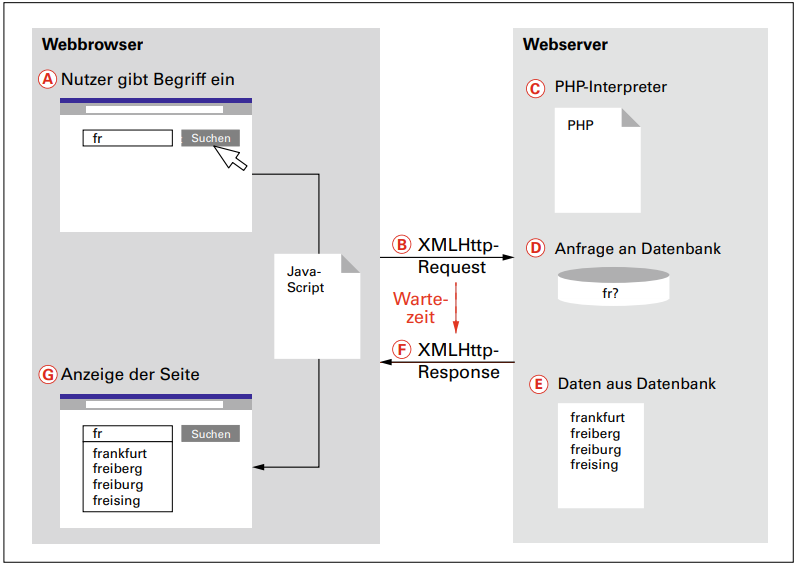
\includegraphics[scale=1.0]{images/AjaxUseCase}
	\caption{Anwendungsfall von Ajax} %TODO Quellenangabe
	\label{img:/AjaxUseCase}
\end{figure}
Während ein User ein Textfeld beschreibt wird im Hintergrund, mithilfe des JavaScript-Objektes XMLHttpRequest, eine Anfrage an den Webserver gesendet. Dieser kann mit ersten Teilergebnissen antworten und so dem User bspw eine Autovervollständigung anbieten. Ajax ist in dem Fall keine neue Technologie sondert verwendet JavaScript anders um mit dem Webserver im Hintergrund zu kommunizieren. In diesem Fall ist die Autovervollständigung lediglich ein einfaches Beispiel um die Funktion von \ac{Ajax} zu verstehen. Darüber hinaus gibt es weitaus mehr Anwendungsfälle von \ac{Ajax}. Bei aufwändigen Webseiten kommt ein weiteres Element zur Webentwicklung hinzu, das die Entwicklung erleichtern soll. Dabei handelt es sich um Frameworks. Wie es für \ac{CSS} Bootstrap als Framework gibt, so werden viele auch im Zusammenhang mit JavaScript angeboten. Eines der beliebtesten Frameworks ist \textbf{jQuery}. Mit jQuery wird das Programmieren von JavaScript unterstützt. Außerdem orientiert es sich an der Darstellung von \ac{CSS} wie bspw. der Zugriff auf ein Element über \$(\dq \#bereich1\dq) oder \$(\dq .farbe1\dq). Wie JavaScript kann auch jQuery auf die Elemente der \ac{HTML}-Seite zugreifen. Der Standardaufbau, welcher in der folgenden Abbildung dargestellt ist, zeigt eine Merkmal auf das zu achten ist.
\begin{lstlisting}[language=HTML,caption=Example Listing of jQuery,label={lst:jQueryExample}]
<script> $(document).ready(function(){
/* Hier der jQuery-Code */ });
</script>
\end{lstlisting}
Mit \textit{\$(document).ready} werden grundsätzlich erste Probleme, die auftreten können verhindert. Demnach könnte ohne diese Funktion auf Elemente zugegriffen werden, welche noch nicht vollständig geladen sind. Das ready verhindert diese Problematik und wartet mit der Ausführung bis die Webseite komplett geladen ist. JQuery besitzt zahlreiche Plugins die bei der Webentwicklung verwendet werden können. JavaScript bildetet ein fundamentaler Baustein, der mithilfe zahlreicher Möglichkeiten und Frameworks für jede Anwendung Optionen bereitstellt, um dynamische Änderungen oder Interaktionen zu integrieren.\cite{buhler2018webtechnologien}


\pagebreak
\section{Grundlagen von Softwaretests}
\label{sec:GrundlagenSoftwaretests}

Die Entwicklung eines Softwareprodukts ist stets aufwendig und fehlerbehaftet. Es gibt eine Reihe potentieller Fehler, die eine Software aufweisen kann.

\smallskip

\textbf{Häufige Fehlerarten:}

\smallskip

\begin{itemize}
\item syntaktische Fehler
\item semantische Fehler
\item Logische Fehler
\item Designfehler
\item Fehler im Bedienkonzept
\item Laufzeitfehler
\item Fehler als Folge physikalischer Betriebsbedingungen
\end{itemize}

Syntaktische Fehler verstoßen gegen die Richtlinien und der Grammatik der Programmiersprache. Bei semantischen Fehlern ist die Syntax korrekt, aber das Programm ist inhaltlich falsch. Ein Beispiel wäre eine falsche Parameterreihenfolge in einer Funktion. Logische Fehler bestehen aus einem falschen Problemlösungsansatz, zum Beispiel aufgrund eines Fehlschlusses oder einer falschen Interpretation einer Programmspezifikation. Designfehler sind Fehler im Grundkonzept der Software. Die Ursachen liegen in der Definition der Anforderungen an das Softwareprodukt oder an Codewiederholungen, die bei Software-Wartungen nicht auf den gleichen Stand gebracht werden. Ein Fehler im Bedienkonzept ist ein Fehler, bei dem sich das Programm anders als von Benutzern erwartet verhält, obwohl es technisch fehlerfrei arbeitet. Laufzeitfehler sind Fehler, die auftreten während das Programm abgearbeitet wird. Ein möglicher Laufzeitfehler entsteht durch einen Aufruf eines Unterprogramms mit falschen Eingabeparametern. Fehler als Folge physikalischer Betriebsbedingungen sind Fehler, die durch elektromagnetische Felder, Temperaturschwankungen oder Strahlung bei technisch einwandfreier Software zu Fehlern und unerwünschten Verhalten führen. Ein Kippen eines Bits auf aufgrund der beschriebenen Einflüsse kann die Ausführung des Programms beeinträchtigen oder abstürzen lassen.\cite{witte2019testmanagement}\\

Syntaktische Fehler können durch den Interpreter oder Compiler schnell identifiziert und behoben werden. Semantische Fehler, logische Fehler und andere Fehlerarten sind schwer zu finden. Die Programmverifikation stellt einen systematischen Ansatz dar, um die Fehlerfreiheit von Programmen zu beweisen. Sie wendet mathematische Beweisführungen, Axiome und Schlussregeln an, um solche Fehler ausschließen zu können.\\
In wenigen modernen Programmiersprachen ist jedoch eine Beweisführung auf Fehlerfreiheit möglich. Die Softwarestrukturen und der Codeumfang wachsen und erschweren die manuelle Beweisführung. Nach dem niederländischen Informatiker Dijkstra E. W. lässt sich ein Programm formal in eine Vor- und Nachbedingung spezifizieren. \autoref{img:VorNachbedingungDijkstra} zeigt den logischen Aufbau eines Programms. Eine Vorbedingung (precondition) ist eine Menge an Zusicherungen, die zu Beginn eines Programms gültig ist. Eine Nachbedingung (postcondition) ist eine Menge an Zusicherungen, die am Ende des Programms gültig sind. Der Begriff Zusicherung (assertion) ist definiert als eine Aussage, die an einer bestimmten Stelle des Programmablaufes gültig ist. Ein Programm ist nach Dijkstra genau dann korrekt, wenn das Programm seine Vorbedingungen in einer endlichen Anzahl an Schritten in seine Nachbedingung überführt. Vor- und Nachbedingungen sind in der Programmspezifikation genau definiert.\cite{kirchner2017}

\begin{figure}[h]
	\centering
	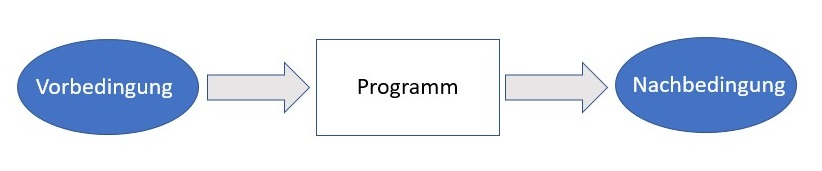
\includegraphics[width=\textwidth]{images/VorNachbedingungDijkstra}
	\caption{Logischer Aufbau eines Programms nach Dijkstra, eigene Darstellung}
	\label{img:VorNachbedingungDijkstra}
\end{figure}

Das einhalten von Vor- und Nachbedingungen ist in moderner Softwareentwicklung stets gefordert. Weil das anwenden von Beweisführungen und Schlussregeln auf Programmen heutzutage zu komplex sind und für den Menschen in komplexen Softwarearchitekturen nur noch schwer nachzuvollziehen sind, wird explizit Code entwickelt, der den entwickelten Code testet. Das führt zur Unterscheidung zwischen Produktions- und Testcode. Der Testcode soll den Produktionscode auf korrektes Verhalten überprüfen.\cite{kirchner2017}

Nach der Auslieferung von Software können Fehler immer noch entdeckt werden, zum Beispiel durch den Kunden. Das bestätigt die These von Dijkstra:

\smallskip

\textbf{\glqq Durch Testen kann man stets nur die Anwesenheit, nie aber die Abwesenheit von Fehlern beweisen.\grqq} (vgl. Dijkstra E. W. - The Humble Programmer, ACM Turing Lecture 1972)

\smallskip

Diese These bestätigt Witte F. in \cite{witte2019testmanagement}. Testaktivitäten schlagen fehl und erzeugen Fehler. Nach \cite{witte2019testmanagement} ist das Risiko, dass noch unentdeckte Fehler im Testobjekt vorhanden sind geringer, je höher die Testabdeckung ist. Testen zeigt nicht, dass die Software fehlerfrei ist, selbst wenn keine Fehler nachgewiesen werden. Testen ist kein mathematischer Beweis. Softwaretests beziehen sich immer auf die Betrachtung von Stichproben, es werden nicht alle möglichen Eingabeparameter und deren Kombinationen mit allen möglichen Vorbedingungen getestet, sondern diejenigen, die am ehesten praxisrelevant sind. Der Testaufwand richtet sich dabei nach Priorität und Risiko. Der Aufwand ist dabei immer mit
dem Nutzen abzugleichen. 

\smallskip

Eine Software vollständig zu testen ist somit unmöglich. Ein Test dient zur Feststellung, ob ein Programm wie in der Spezifikation festgehalten
funktioniert und nichts anderes tut, aber nicht um alle möglichen Fehler ausschließen zu können.

\smallskip

Tests eines komplexen Software-Systems lassen sich in verschiedene Testarten einordnen. Nicht jeder Test ist in jedem Entwicklungsstand möglich. Weil aber nicht jede Teststufe oder Testart zu jedem Zeitpunkt möglich ist, müssen die Testarten eindeutig voneinander abgegrenzt werden.

\textbf{Testarten:}

\begin{figure}[h]
	\centering
	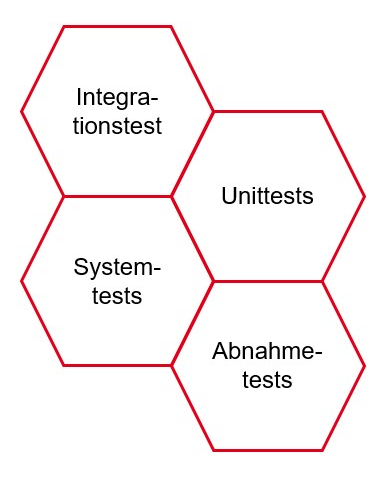
\includegraphics[width=6cm]{images/Testarten.png}
	\caption{Übersicht über Testarten, eigene Darstellung}
	\label{img:Testarten}
\end{figure}

Die häufigsten Testarten lassen sich in vier Bereiche aufteilen - Integrationstests, Unittests, Systemtests und Abnahmetests, siehe \autoref{img:Testarten}. \textbf{Integrationstests} sind abgestimmte Reihen von mehreren Tests, die dazu dienen, verschiedene voneinander abhängige Komponenten eines komplexen Systems im Zusammenspiel miteinander zu prüfen. Für den Integrationstest erstellt man nun Testszenarien, die das Zusammenwirken der beiden betroffenen Komponenten zeigen. Die Anzahl der Integrationsstufen richtet sich nach der Komplexität der Software. \textbf{Systemtests} werden durchgeführt, um die gesamte Software gegen die gesamten Anforderungen des Kunden zu testen. Das beinhaltet alle funktionalen Anforderungen und nicht funktionalen Anforderungen, wie zum Beispiel Qualität oder Bedienbarkeit. Weil Systemtests die gesamte Software testen, sind diese zum Zeitpunkt der Fertigstellung der Software durchzuführen. Idealerweise wird die Produktivumgebung des Kunden zuerst nachgestellt und die Software mit Live-Szenarien aus dem Produktivbetrieb getestet. Ein \textbf{Abnahmetest}, \textbf{Verfahrenstest}, \textbf{Akzeptanztest} oder auch \textbf{User Acceptance Test} ist ein Test der ausgelieferten Software durch den Kunden und/oder Auftraggeber. Der Test wird oft mit Kopien von Echtdaten in der Produktionsumgebung des Kunden durchgeführt. Diese Testart hat nicht das Ziel Fehler zu entdecken, sondern das der Kunde Vertrauen in das Endprodukt gewinnt. Fehler sollten schon durch andere Testarten entdeckt worden und behoben sein. Zum Beispiel durch \textbf{Unittests}. Unittests eignen sich dafür, bei jedem Entwicklungsstand einzusetzen. Diese Art von Tests werden in der Softwareentwicklung durchgeführt, um kleine, funktionale Einzelteile (\textbf{Units}) zu testen. Ein \textbf{Unit} kann dabei ein kleiner Codeabschnitt sein oder eine Methode einer Klasse sein. Weil Algorithmen auf Modulebene meist nur eine begrenzte Komplexität aufweisen und über klar definierte Schnittstellen aktiviert werden, können sie mit relativ wenigen Testfällen ziemlich umfassend getestet werden.\cite{witte2019testmanagement}

\smallskip

Eine wichtige Anforderung an Tests ist, dass diese schnell und effizient ablaufen. Effizient, um nicht mehr als die notwendigen Ressourcen zu verbrauchen und schnell, um möglichst oft aufgerufen zu werden.\cite{hubertz2016softwaretests} Diese Anforderungen erfüllen vor allem Unittests, weshalb für die Entwicklung der Softwarefunktionalitäten des Projekts Unittests eingesetzt werden. Diese werden im nächsten Kapitel genauer erläutert. 

\subsection{Unittests}
\label{Unittests}

\chapter{Umsetzung und Implementierung}
\label{chap:Umsetzung}

\section{Vorbereitung}
\label{sec:Vorbereitung}

\section{Implementierung des Chatservers ejabberd}
\label{sec:ChatserverEntwicklung}

\subsection{Anbindung des Chatservers}
\label{subsec:Anbindung}

\subsection{Security}
\label{subsec:Security}

\subsection{Konfiguration von ejabberd}
\label{subsec:Konfiguration}

\newpage

\section{Entwicklung des Chat-Clients}
\label{sec:ClientEntwicklung}

\ac{HTML}

\subsection{Entwicklung der GUI}
\label{subsec:EntwicklungGUI}

\subsection{Implemintierung des Backends}
\label{subsec:Backend}

\newpage

\chapter{Datenanalyse}
\label{chap:Datenanalyse}

\newpage

\chapter{Ergebnis}
\label{chap:Ergebnis}

\newpage

\chapter{Fazit}
\label{chap:Fazit}


\end{onehalfspacing}
\newpage

\bibliography{Literatur}
\newpage
%setze Anhang mit appendix
%addpart, sodass Anhang im Inhaltsverzeichnis ohne Buchstaben auftaucht
\appendix
\addpart{Anhang}

\chapter{Installation eines Apache Kafka Systems}
\label{InstallationKafka}

Die nachfolgende Anleitung bezieht sich auf die Installation eines Kafka-Systems. Die Installationsanleitung beschreibt alle notwendigen Schritte, um einen Server mit der \textbf{Kafka Version 2.4.0} in Betrieb zu nehmen. Die Anleitung beschreibt nicht, wie ein Cluster-System, welches einen Verbund mehrerer Kafka-Instanzen darstellt, in Betrieb genommen werden kann. Ziel ist es, eine einfache Installation aufzuzeigen und Kafka als Service auf einem Server bereitzustellen ohne, dass für die Ausführung der Kafka-Instanz ein Benutzer angemeldet sein muss. Die Informationen und Befehle sind aus der Kafka-Dokumentation \cite{kafkaDoc} zu entnehmen.

\bigskip

\textbf{Voraussetzungen:}

\smallskip

\begin{itemize}
\item Linux Ubuntu 18.04 LTS
\item Server
\begin{itemize}
\item mindestens 4GB RAM, empfohlen 8GB (Installation mit weniger RAM kann zu Problemen beim Start von Kafka führen, weil die Java Virutal Machine (JVM) eine \glqq OutOfMemory\grqq -Exception werfen kann.
\end{itemize}
\item OpenJDK 8 (Kafka ist in der Programmiersprache Java programmiert und benötigt deshalb eine lauffähige JVM.)
\end{itemize}

\section{Schritt 1: Anlegen eines Benutzers}

Für die Erstellung eines Benutzers muss sich auf dem Server mit einem Benutzer eingeloggt werden. Mit folgendem Kommando wird ein Benutzer mit dem Namen Kafka angelegt. Mit dem zweiten Kommando wird der Benutzer der \glqq sudo\grqq -Gruppe hinzugefügt und ist ab diesem Zeitpunkt berechtigt höher privilegierte Befehle auszuführen. Das letzte Kommando legt ein Passwort an, dass bei der Ausführung höher privilegierter Befehle abgefragt wird.

\smallskip

\begin{lstlisting}[language=Bash]
$ sudo adduser kafka # Benutzer anlegen
$ sudo adduser kafka sudo # Benutzer zur sudo-Gruppe hinzufügen
$ sudo passwd kafka # Anlegen eines sudo-Passwords
\end{lstlisting}

Anschließend muss sich mit dem neu erstellten Benutzer eingeloggt werden (Kommando: su kafka).

\section{Schritt 2: Installation der benötigten Komponenten}


Als nächstes muss das komprimmierte Kafka-Binary heruntergeladen werden. Hierzu kann das \textbf{curl}-Kommandozeilentool verwendet werden, um das Binary direkt aus dem Internet herunterzuladen und im Home-Verzeichnis des kafka-Benutzers gespeichert werden.

\smallskip

\begin{lstlisting}[language=Bash]
$ curl "http://mirror.checkdomain.de/apache/kafka/2.4.0/kafka_2.12-2.4.0.tgz" -o ~/kafka_2.12-2.4.0.tgz
\end{lstlisting}

Falls OpenJDK 8 noch nicht installiert ist, muss folgender Befehl ausgeführt werden.

\smallskip

\begin{lstlisting}[language=Bash]
$ sudo apt-get install openjdk-8-jdk
\end{lstlisting}

Erstellen Sie ein Grundverzeichnis in dem alle Kafka-Komponenten extrahiert werden können. Legen Sie mit folgendem Befehl ein Verzeichnis mit dem Namen \glqq kafka\grqq an. Extrahieren Sie die komprimierte Datei in dasselbe Verzeichnis.

\smallskip

\begin{lstlisting}[language=Bash]
$ mkdir ~/kafka && cd ~/kafka
$ tar -xvzf ~/kafka_2.12-2.4.0.tgz --strip 1
\end{lstlisting}

Kafka ist ab jetzt bereit für eine Konfiguration.

\section{Schritt 3: Konfiguration von Kafka}

Kafka lässt es in der Standardkonfiguration nicht zu neue Topics, eine Kategorie oder eine Gruppe zu löschen. Um das zu ändern, muss die Konfigurationsdatei von Kafka angepasst werden. Falls der \glqq nano\grqq -Editor auf Ihrem System nicht verfügbar ist, können Sie einen Editor Ihrer Wahl verwenden, zum Beispiel \glqq vi\grqq.

\smallskip

\begin{lstlisting}[language=Bash]
$ nano ~/kafka/config/server.properties
\end{lstlisting}

Fügen Sie diese Einstellung in der Datei hinzu:

\textbf{delete.topic.enable = true}

Speichern Sie anschließend die Datei und beenden Sie den Editor.

Kafka benötigt \textbf{Zookeeper}, um erfolgreich starten zu können. Zookeeper ist automatisch nach der Installation aus Schritt 2 vollständig vorhanden und befindet sich ebenfalls im erstellten \glqq kafka\grqq -Verzeichnis. Testen Sie mit folgenden Kommandos, ob Zookeeper und Kafka erfolgreich starten. Starten Sie zuerst Zookeeper, warten Sie 30 Sekunden, öffnen Sie eine zweite CLI auf dem System und starten Sie anschließend Kafka. Wird kein Fehler geworfen, waren alle Schritte bisher erfolgreich verlaufen und Kafka ist betriebsbereit.

\smallskip

\begin{lstlisting}[language=Bash]
$ ~/kafka/bin/zookeeper-server-start.sh ~/kafka/config/zookeep.properties # Start: zookeeper
$ ~/kafka/bin/kafka-server-start.sh ~/kafka/config/server.properties # Start: kafka
\end{lstlisting}

Zeigt der Kommandozeilen-Output nur Nachrichten der Kategorie \glqq INFO\grqq und keine Fehlermeldungen, sind beide Dienste erfolgreich gestartet. Ansonsten überprüfen Sie Ihre Schritte erneut und korrigieren Sie die Fehler.

Für den Start von Kafka ist im aktuellen Zustand eine Anmeldung des Benutzers erforderlich, der Zookeeper und Kafka als Benutzerprozess startet. Um Kafka als Server-Dienst bereitzustellen folgen Sie dem nächsten Kapitel der Anleitung. Möchten Sie lediglich die Grundfunktionalitäten ausprobieren und benötigen keine globale Verfügbarkeit, kann Schritt 4 der Anleitung entfallen.

\section{Schritt 4: Bereitstellung von Kafka als Server-Dienst}

Teilschritte für die Bereitstellung als Server-Dienst:

\begin{itemize}
\item Systemd-Datei für Zookeeper erstellen
\item Systemd-Datei für Kafka erstellen
\item Zookeeper-Dienst starten
\item Kafka-Dienst starten
\end{itemize}

\bigskip

\textbf{Systemd-Datei für Zookeeper erstellen:}

\bigskip

\begin{lstlisting}[language=Bash]
$ sudo nano /etc/systemd/system/zookeeper.service
\end{lstlisting}

Folgender Inhalt muss in die Datei kopiert werden:

\smallskip

\begin{lstlisting}[language=Bash]
[Unit]
Requires=network.target remote-fs.target
After=network.target remote-fs.target

[Service]
Type=simple
User=kafka
ExecStart=/home/kafka/kafka/bin/zookeeper-server-start.sh /home/kafka/kafka/config/zookeeper.properties
ExecStop=/home/kafka/kafka/bin/zookeeper-server-stop.sh
Restart=on-abnormal

[Install]
WantedBy=multi-user.target
\end{lstlisting}

Speichern Sie die Datei und gehen Sie zum nächsten Schritt.

\pagebreak

\textbf{Systemd-Datei für Kafka erstellen:}

\bigskip

\begin{lstlisting}[language=Bash]
$ sudo nano /etc/systemd/system/kafka.service
\end{lstlisting}

Folgender Inhalt muss in die Datei kopiert werden:

\smallskip

\begin{lstlisting}[language=Bash]
[Unit]
Requires=zookeeper.service
After=zookeeper.service

[Service]
Type=simple
User=kafka
ExecStart=/bin/sh -c '/home/kafka/kafka/bin/kafka-server-start.sh /home/kafka/kafka/config/server.properties > /home/kafka/kafka/kafka.log 2>&1'
ExecStop=/home/kafka/kafka/bin/kafka-server-stop.sh
Restart=on-abnormal

[Install]
WantedBy=multi-user.target
\end{lstlisting}

Speichern Sie die Datei und gehen Sie zum nächsten Schritt.

\textbf{Zookeeper-Dienst starten:}

\bigskip

\begin{lstlisting}[language=Bash]
$ sudo systemctl start zookeeper # Starten des Zookeeper-Dienstes
\end{lstlisting}

Überprüfen Sie den Status des Diensts mit folgendem Kommando. Der Status sollte \glqq active\grqq sein.

\smallskip

\begin{lstlisting}[language=Bash]
$ sudo systemctl status zookeeper
\end{lstlisting}

Der Output zeigt, dass Zookeeper erfolgreich gestartet wurde:

\begin{figure}[h]
	\centering
	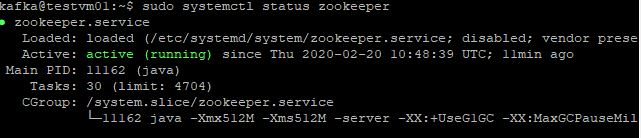
\includegraphics{images/StatusZookeeper}
	\caption{Status des Zookeeper-Dienstes nach dem Start}
	\label{img:StatusZookeeper}
\end{figure}

Für ein automatisches Starten des Dienstes nach einem Reboot führen Sie folgendes Kommando aus:

\smallskip

\begin{lstlisting}[language=Bash]
$ sudo systemctl enable zookeeper
\end{lstlisting}

Ab jetzt wird Zookeeper automatisch nach einem Neustart beim Hochfahren aller Systeme mit gestartet.

\pagebreak

\textbf{Kafka-Dienst starten:}

\bigskip

Führen Sie die gleichen Befehle für den Start des Kafka-Dienstes durch. Achten Sie darauf, dass Sie in allen Befehlen \glqq zookeeper\grqq durch \glqq kafka\grqq als Dienstbezeichnung ersetzen.

\smallskip

Überprüfen Sie mit dem \glqq status\grqq -Befehl, ob der Dienst richtig gestartet wurde. Der Output sollte so aussehen:

\begin{figure}[h]
	\centering
	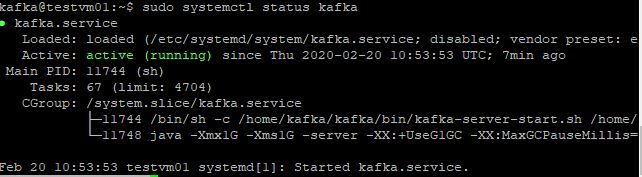
\includegraphics{images/StatusKafka}
	\caption{Status des Kafka-Dienstes nach dem Start}
	\label{img:StatusZookeeper}
\end{figure}

Nun sind Zookeeper und Kafka als Linux-Server-Dienst verfügbar ohne, dass ein Benutzer hierfür dauerhaft angemeldet sein muss.

\section{Schritt 5: Testen der Installation}

Um sicherzustellen, dass Kafka als Dienst korrekt läuft, wird eine \glqq HelloWorld\grqq -Nachricht produziert und konsumiert. Um eine Nachricht mittels Kafka zu versenden sind zwei Bestandteile nötig:

\begin{itemize}
\item Producer, welcher ein Topic registriert und Nachrichten produziert
\item Consumer, welcher Nachrichten aus dem Topic lesen kann
\end{itemize}

Hierfür werden die bei der Installation mitgelieferten Skripte im \glqq kafka\grqq -Verzeichnis benutzt.

Zuerst muss ein Topic erstellt werden. Das Topic heißt für Testzwecke \glqq Test\grqq.  Führen Sie folgenden Befehl aus:

\smallskip

\begin{lstlisting}[language=Bash]
$ ~/kafka/bin/kafka-topics.sh --create --zookeeper localhost:2181 --replication-factor 1 --partitions 1 --topic Test
\end{lstlisting}

Der Befehl benötigt den Zookeeper-Dienst mit dessen Portnummer (Standard-Port: 2181) als Argument, weil Zookeeper für die Verwaltung der Kafka-Instanzen benötigt wird. Ist das Topic erfolgreich erstellt worden, ist der Output auf der Kommandozeile \glqq Created topic Test.\grqq

\pagebreak

Um einen Producer zu starten, der als Nachricht \glqq HelloWorld\grqq produziert und dem Kafka-Dienst übergibt, führen Sie folgenden Befehl aus:

\smallskip

\begin{lstlisting}[language=Bash]
$ echo "Hello, World" | ~/kafka/bin/kafka-console-producer.sh --broker-list localhost:9092 --topic Test > /dev/null
\end{lstlisting}

Der Befehl produziert eine Nachricht für das Topic \glqq Test\grqq und übergibt die Nachricht an Kafka.

Der Consumer benötigt als Argument den Zookeeper Hostname und den Port (Standardport: 2181) und das Topic aus dem Nachrichten konsumiert werden sollen.

\smallskip

\begin{lstlisting}[language=Bash]
$ ~/kafka/bin/kafka-console-consumer.sh --bootstrap-server localhost:9092 --topic Test --from-beginning
\end{lstlisting}

Nach der Ausführung des Consumer-Skripts, sollte die Nachricht \glqq HelloWorld\grqq auf dem Bildschirm erfolgen. Ist das nicht der Fall, überprüfen Sie Ihre durchgeführten Schritte. Das Skript blockiert den Benutzerprozess, weil der Consumer weiterhin auf eintreffende Nachrichten wartet. Um das Skript abzubrechen verwenden Sie STR+C als Shortcut auf der Tastatur.

Kafka steht nun als Server-Dienst zur Verfügung und die Installation wurde durch einen Test erfolgreich validiert. Kafka kann für seine Einsatzbereiche ab jetzt vollständig verwendet werden.

\end{document}